% Created 2023-01-30 lun 14:35
% Intended LaTeX compiler: pdflatex
\documentclass[openany, a4paper]{book}
\usepackage[utf8]{inputenc}
\usepackage[T1]{fontenc}
\usepackage{graphicx}
\usepackage{longtable}
\usepackage{wrapfig}
\usepackage{rotating}
\usepackage[normalem]{ulem}
\usepackage{amsmath}
\usepackage{amssymb}
\usepackage{capt-of}
\usepackage{hyperref}
\usepackage{amsmath,amssymb,amsthm,geometry,hyperref,paralist,svg,thmtools,tikz,tikz-cd}
\usepackage{mathtools}
\usepackage[capitalise,noabbrev]{cleveref}
\usepackage{mdframed} \usepackage{svg}
\usepackage{environ} \NewEnviron{abmn}{\marginnote{\BODY}}
\usepackage{url}
\usepackage{color}
\usepackage{listings,chngcntr}% http://ctan.org/pkg/listings
\usepackage{multicol}
\usepackage{url}
\usepackage{tabularx}
\lstset{ basicstyle=\ttfamily, mathescape=true, frame=Trbl, numbers=left}
\renewcommand{\lstlistingname}{Pseudocódigo}
\setcounter{tocdepth}{1}
\newtheoremstyle{break}{\topsep}{\topsep}{\itshape}{}{\bfseries}{}{\newline}{}
\theoremstyle{break}
\newtheorem{theorem}{Theorem}
\newtheorem{corollary}[theorem]{Corollary}
\newtheorem{proposition}[theorem]{Proposition}
\newtheorem{definition}[theorem]{Definition}
\newtheorem{lemma}[theorem]{Lemma}
\newtheorem{affirmation}[theorem]{Affirmation}
\theoremstyle{example}
\newtheorem{example}{Example}
\newtheorem{exmpl}{Example}
\theoremstyle{note}
\newtheorem{note}{Note}
\theoremstyle{break}
\newtheorem{remark}{Remark}
\theoremstyle{exercise}
\newtheorem{exercise}{Exercise}
\usetikzlibrary{arrows,automata,positioning}
\NewEnviron{obs}{\begin{mdframed}\begin{remark} \BODY \end{remark}\end{mdframed}}
\NewEnviron{nota}{\begin{mdframed}\begin{note} \BODY \end{note}\end{mdframed}}
\renewcommand{\qedsymbol}{\textbf{\therefore}}
\NewEnviron{blk}{\begin{mdframed}\BODY\end{mdframed}}
\newcommand{\nimplies}{\;\not\nobreak\!\!\!\!\implies}
\AtBeginDocument{\renewcommand{\thelstlisting}{\thesection.\arabic{lstlisting}}}
\AtBeginDocument{\counterwithin{lstlisting}{section}}
\newcommand{\R}{{\sf \small Read}\xspace}
\newcommand{\W}{{\sf \small Write}\xspace}
\author{Miguel Angel Piña Avelino}
\date{\today}
\title{A Study Of Concurrent Data Structures With Relaxed Semantics}
\hypersetup{
 pdfauthor={Miguel Angel Piña Avelino},
 pdftitle={A Study Of Concurrent Data Structures With Relaxed Semantics},
 pdfkeywords={},
 pdfsubject={},
 pdfcreator={Emacs 28.2 (Org mode 9.5.5)},
 pdflang={Spanish}}
\begin{document}

\maketitle
\tableofcontents


\chapter{Introduction}
\label{sec:orgc028e86}

\section{About Concurrent Computing}
\label{sec:orga3fcb79}

What is concurrent computing? This is a good question. We should first talk
about single-core and multi-core processors manufactured by the computer
industry. After the second world war and until the 90's the general purpose
cpus were single-core. All processes were executed in a single-core, and the
operating systems simulated concurrency using schedulers and other
techniques. In 2001, IBM introduce the first multi-core processor
\cite{ibmIBM100Power}, it allows that two processors work together at a very
high bandwidth (for the epoch) with large on-chip memories and with
high-speed buses. Since then, the amount of cores in each processors has been
increasing. We must consider as well the Moore's law, loosely speaking, this
law tells us that each year more and more transistors are placed into the
same space (i.e. electronic components and circuits are reduced in size), but
their speed cannot be increased without overheating. Consequently, the
industry move to ``multi-core'' architectures. In this architecture multiple
processors communicate through shared memory (RAM, hardware caches),
permitting make computing more effectively using \emph{parallelism}, where the
processors work together on a single task \cite{DBLP_books_daglib_0020056}.

\subsection{Classic concurrent computing}
\label{sec:org8522a58}

\begin{itemize}
\item[{$\square$}] Basic Definitions
\item[{$\square$}] FLP impossibility result
\item[{$\square$}] Asynchronous Shared Memory
\item[{$\square$}] Primitive Synchronization Operations and Consensus
\end{itemize}

\subsection{Relaxed concurrent computing}
\label{sec:orgf751443}

\begin{itemize}
\item[{$\square$}] Relaxing the problem
\item[{$\square$}] Multiplicity preliminaries
\item[{$\square$}] Another relaxations?
\end{itemize}

\subsection{Work-stealing}
\label{sec:orgc2b91c1}

\begin{itemize}
\item[{$\square$}] How it works the work-stealing
\item[{$\square$}] Classic algorithms
\item[{$\square$}] Idempotent algorithms
\item[{$\square$}] Work-stealing with multiplicity
\end{itemize}

\subsection{Data-Structures}
\label{sec:org24d5250}

\begin{itemize}
\item[{$\square$}] Queues with multiplicity
\item[{$\square$}]
\end{itemize}

\subsection{Contributions}
\label{sec:org8f806d2}

\subsection{Organization}
\label{sec:orgac63711}


\section{Preliminaries}
\label{sec:org5aa7654}


\subsection{Mathematical model}
\label{sec:org7079ef2}


\subsection{Realistic model of computation}
\label{sec:org6fb4494}

We consider a standard concurrent shared memory system with \(n \ge 2\)
\emph{asynchronous} processes, \(p_0, \ldots, p_{n-1}\), which may crash at any time
during an execution. The processes communicate with each other by invoking
atomic instructions of base objects: either simple Read/Write instructions to
\textbf{atomic objects}, or more powerful \textbf{Read-Modify-Write} instructions, such as
\texttt{Test-And-Set}, \texttt{Swap} or \texttt{Compare-And-Set}.

For simplicity we assume a single multicore chip where the processes run. In
our system we consider a memory hierarchy, where we have the following
elements in the hierarchy:

\begin{itemize}
\item Cache memory
\item Memory bus
\item Main memory
\end{itemize}

In this model, each processor core may read and
write to a single shared memory space. Usually each processor core has a
cache to operate with data from the shared memory. Often, this data is
transferred through a memory bus, allowing connect the processors with the
memory. The figure \ref{fig:arch} shows a simplified view of this model. In
the sections: \hyperref[sec:orgffc38d9]{Cache memory}, \hyperref[sec:org01f40e0]{Memory bus} and \hyperref[sec:org740f1d9]{Main memory}, we explain more in
detail the meaning of each bullet of the list.

\begin{figure}
\begin{minipage}{\linewidth}
  \includesvg[width=\linewidth]{figs/architecture}
\end{minipage}
\caption{Simplified view of a modern computer system cache architecture}
\label{fig:arch}
\end{figure}


\subsection{Cache memory}
\label{sec:orgffc38d9}

The cache memory is a special very high-speed memory that is very close to
the processor and the processes can access it very fast. The caches are used
to reduce average latencies to access storage structures
\cite{DBLP_series_synthesis_2020Nagarajan}. In recent multicore chips, the
cache memory is divided in three levels, two private levels (L1 and L2) for
each processor and a third level (L3) that is shared by the cores. The
purpose of the first two levels is to provide fast access to data and
instructions for the processors.

Each processor use the first level of cache to get the data and instructions
to execute them, usually the access to this level of cache is very fast
respect to the access to other levels.  The second level is often more
capacious than first level and is used to store data and instructions that
are close to be executed. In the third level, this cache is shared by many
processors and is used as feeder for the L2 cache.

\subsection{Memory bus}
\label{sec:org01f40e0}

Is a computer bus that allows transfer data from the primary memory to the
CPU and the cache memory. It is made up of two parts: the data bus and the
address bus. The data bus is in charge of transfer information between the
primary memory and the correspondent chipset.
The address bus is used to retrieve information about the location of stored
information.


\subsection{Main memory}
\label{sec:org740f1d9}

Is the responsible of hold the data that CPU need to access frequently, such
as instructions or data currently being processed. The CPU can access to
this information faster than the access to secondary memory.

\subsection{Consistency Memory Model and Cache Coherence}
\label{sec:org4c45d72}

\begin{enumerate}
\item Consistency memory model
\label{sec:org6756469}

Following the simplified view of the cache architecture, we want to have a
correct shared memory. And what this means? The correctness of the shared
memory can be separated into two sub-issues: \emph{consistency} and \emph{correctness}.

The consistency (definitions) provide rules about loads and stores (memory
reads and writes) and how they act upon memory. These definitions must take
into account the behaviour of those operations on memory through access of
multiple threads or even a single thread. The consistency models define
correct shared memory behavior in terms of loads and stores, without
reference to caches or coherence \cite{DBLP_series_synthesis_2020Nagarajan}.
Shared memory correctness is specified by a memory consistency model (or
memory model). This specifies the allowed behavior of multithreaded programs
executing with shared memory.

The most intuitive and strongest memory model is the \emph{Sequential Consistency}
(SC). Another memory model used by systems \emph{x86} and \emph{SPARC} is \emph{Total Store Order}
(TSO), motivated by the desire of use \emph{first-in-first-out} write buffers to
hold the results of committed stores before writing results to the caches.
Additional to the prior memory model, "relaxed" or "weak" memory models are
considered, because these models shows that most memory orderings in strong
models are unnecessary \cite{DBLP_series_synthesis_2020Nagarajan}.

\item Cache coherence
\label{sec:org7d8c51f}

Cache coherence protocols are used in response to solve a coherence problem
in cache. For example, a coherence problem can arise if multiple cores have
access to multiple copies of a datum, each one in a core, and at least one
them is a write access. The cache coherence protocols prevent the access to
stale data (incoherent data); this can be done using a set of rules
implemented by the distributed set of cores within a system. These
protocols use the common MOESI coherence states: modified (M), owned (O),
exclusive (E), shared (S) and invalid (I). The protocol acts like a state
machine, moving from one state to another based on the conditions of the
data and the cache memory \cite{DBLP_series_synthesis_2020Nagarajan}.
\end{enumerate}



\subsection{Memory fences}
\label{sec:org76782bc}

A memory fence is a barrier instruction that causes a CPU or compiler to
enforce a an ordering constraint on memory operations (loads and stores)
issued before and after the barrier instruction.

These instructions are necessary because most modern CPUs or compilers
employ performance optimizations, changing the order of the instructions on
one program, that could result in out-of-order execution. Normally these
optimizations are unnoticed in a single thread program, but can cause an
unpredictable behavior in concurrent programs.

For example, consider the following multi-thread program, with 2
threads, each one running in one core in a concurrent way:

Thread 1, core 1
\begin{verbatim}
while (z == 0);
print(y);
\end{verbatim}

Thread 2, core 2
\begin{verbatim}
y = 30;
z = 1;
\end{verbatim}

In this case, we might expect that the \texttt{print(y)} always print the number 30,
nevertheless, the compiler or the CPU could change the order of the
instructions for the thread 2, giving as result an execution where the value
for \texttt{y} is undefined and the instructions could be interleaved as follows:

\begin{verbatim}
z = 1; // Thread 2
while (z == 0); // Thread 1
print(y); // Thread 1
y = 30; // Thread 2
\end{verbatim}

This execution is sequentially consistent, but is an out-of-order
execution producing an undefined result. With the use of memory barriers, we
can ensure that instructions don't be reordered. For example, our code could
be rewrite as follows:

Thread 1, core 1.
\begin{verbatim}
while (z == 0);
fence()
print(y);
\end{verbatim}

Thread 2, core 2.
\begin{verbatim}
y = 30;
fence();
z = 1;
\end{verbatim}


Languages as \texttt{Java} or \texttt{C++} provide instructions to establish synchronization
and ordering constraints between threads without an atomic operation. These
instructions have semantics well defined for

In the case of Java, we have static methods of the class VarHandle
(\texttt{java.lang.invoke.VarHandle}) that are refered as memory fence methods which
helps to provide fine-grained control of memory ordering. These statics
methods are \cite{varHandleJdk92017}:

\begin{description}
\item[{fullFence}] Ensures that loads and stores before the fence will not be
reordered with loads and stores after the fence. This method has memory
ordering effects compatible with
\texttt{atomic\_thread\_fence(memory\_order\_seq\_cst)}.
\item[{acquireFence}] Ensures that loads before the fence will not be reordered
with loads and stores after the fence. This method has memory ordering
effects compatible with \texttt{atomic\_thread\_fence(memory\_order\_acquire)}.
\item[{releaseFence}] Ensures that loads and stores before the fence will not
be reordered with stores after the fence. This method has memory ordering
effects compatible with \texttt{atomic\_thread\_fence(memory\_order\_release)}.
\item[{loadLoadFence}] Ensures that loads before the fence will not be
reordered with loads after the fence.
\item[{storeStoreFence}] Ensures that stores before the fence will not be
reordered with stores after the fence.
\end{description}

For C++, we have the function
\texttt{std::atomic\_thread\_fence}\cite{threadFenceCpp2020}, which establishes
memory synchronization ordering of non-atomic and relaxed atomic access, as
instructed by order, without an associated atomic operation. The type of
synchronization that can handle are the following:

\begin{itemize}
\item Fence-atomic synchronization
\item Atomic-fence synchronization
\item Fence-Fence Synchronization
\end{itemize}

And using a memory order\cite{memoryOrderCpp2020}, it can specifies how
memory accesses, including regular, non atomic memory accesses, are to be
ordered around an atomic operation. In total are six orders, from the
relaxed memory order to the sequential consistent memory order. They are:
\texttt{memory\_order\_relaxed}, \texttt{memory\_order\_consume}, \texttt{memory\_order\_acquire},
\texttt{memory\_order\_acq\_rel} and \texttt{memory\_order\_seq\_cst}. A note about
\texttt{atomic\_thread\_fence} functions, is that on x86 (x86\textsubscript{64}), these functions
issue no CPU instructions and only affect compile time code, with exception
for \texttt{std::atomic\_thread\_fence(std::memory\_order::seq\_cst)}, which issue the
full memory fence instruction \texttt{MFENCE}. For other archict



\section{Work-Stealing}
\label{sec:org05e3761}

We analyze the algorithms for work-stealing described in the article Fully
Read/Write Fence Free Work-Stealing With Multiplicity, also the algorithm
called "Idempotent FIFO Work-Stealing", this because the algorithm have a
similar semantic than the prior algorithms.

\begin{figure}
\begin{minipage}{\linewidth}
  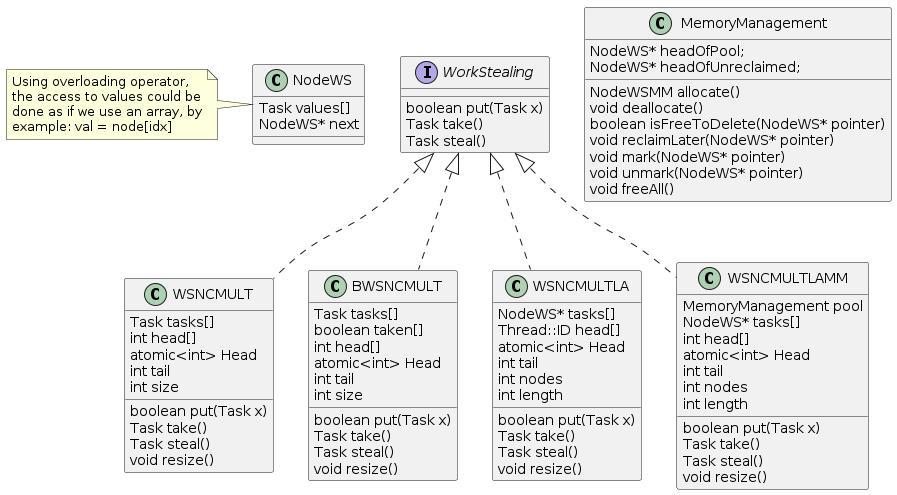
\includegraphics[width=\linewidth]{figs/objects.png}
\end{minipage}
\caption{Simplified view of a modern computer system cache architecture}
\label{fig:arch}
\end{figure}


\subsection{Model}
\label{sec:org98cf114}

\subsection{Known algorithms}
\label{sec:org7f7ca03}

\subsection{Pseudocode for Work-Stealing with Weak Multiplicity}
\label{sec:org805f12a}



\section{Data-Structures}
\label{sec:org772c269}

\subsection{Queues}
\label{sec:orgd7f54ef}

\subsection{Stacks}
\label{sec:org78ed28c}


\section{Some Hardware Foundations}
\label{sec:org2ebf004}

\subsection{Cache memory}
\label{sec:orgb86d5a2}

The cache memory

\begin{enumerate}
\item Multiple caches
\label{sec:orgf9fa5aa}


\item Cache coherence protocols
\label{sec:org6ea87d1}



\begin{enumerate}
\item MESI
\label{sec:orgda5713f}


\item MOESI
\label{sec:orgc59ea28}
\end{enumerate}


\item Store Buffers
\label{sec:orgcc878dd}
\end{enumerate}


\subsection{Reordering (CPU or Compiler)}
\label{sec:org78df52e}


\subsection{Memory Barriers}
\label{sec:org4f6cbbd}


\begin{enumerate}
\item X86 and TSO architectures
\label{sec:org51e1fb1}


\item Memory Fences
\label{sec:orgbd3dc5e}
\end{enumerate}


\subsection{Read-Modify-Write Operations}
\label{sec:org3ee454b}


\subsection{Bibliography}
\label{sec:org0c15272}

\begin{itemize}
\item \url{https://blog.the-pans.com/std-atomic-from-bottom-up/}
\end{itemize}


\subsection{Memory management}
\label{sec:org9b8c916}

To implement efficiently the idempotent algorithms in an enviroment without
garbage collection, it's necessary use some technique or metodology to
provide garbage collection when atomic pointers are used or when distinct
threads want to reclaim the memory of the object associated to the pointer.

\begin{enumerate}
\item Strategies to delete shared pointers
\label{sec:orgd215657}

\begin{itemize}
\item Add pointers to list to safety delete.
\item Do this when there aren't more threads accessing to methods.
\begin{itemize}
\item Increase the counter when a thread enter to the method and decrease when
it exits.
\item Delete all pointers when the counter be equal to zero.
\end{itemize}
\end{itemize}


\item Hazard pointers
\label{sec:orgc0db5d7}

The \emph{Hazard Pointers} is a technique to manage memory in languages where there
are not a garbage collector. This technique was proposed by Maged
Michael \cite{DBLP_journals_tpds_Michael04}. They are so called because
deleting a pointer that might be referenced by other thread(s) is
dangerous. If another threads keep holding references to that pointer and
proceed to access to that pointer after be deleted, you have a undefined
behavior \cite{DBLP_journals_tpds_Michael04}.

The basic idea of this technique is the following:

\begin{itemize}
\item If a thread want to use a pointer that another thread might want to
delete, it first sets a hazard pointer to the pointer, informing to the
other thread that deleting the pointer would be dangerous. Once the object
is not longer needed, the hazard pointer is cleared.
\item When a thread wants to delete the pointer, it must check if the hazard
pointers belonging to the other threads in the system. If no one has a
reference to the pointer, then, it's safe to delete the
pointer. Otherwise, it must be left until later.
\item Periodically, we must check the list of objects that have been left until
later to see if any of them can be deleted now.
\end{itemize}

A general pseudocode for this technique could be the following:

\begin{verbatim}
void func() {
    std::atomic<void*>& hp = get_hazard_pointer_for_current_thread();
    void* old_data = data.load();
    do {
        void* temp;
        do{ // Loop until you've set the hazard pointer
            temp = old_data;
            hp.store(old_data);
            old_data = data.load();
        } while (old_data != temp);
          }while (old_data &&
            !data.compare_exchange_strong(old_data, old_data->next);
    // Do something with old_data
    hp.store(nullptr); // clearing usage of hazard pointer
    // Trying clearing
    if (outstanding_hazard_pointers_for(old_head))
    {
        reclaim_later(old_data);
    }
    else
    {
        delete old_data;
    }
    delete_nodes_with_no_hazards();
}
\end{verbatim}


\item Atomic Smart Pointers (Herlihy, Chapter 19) (Not available for GCC and CLang)
\label{sec:org23fd36b}


When a memory region is reclaimed, the programmer cannot know how that
region of memory will be reused or if even whether it is reused. We need a
way of developing a (general) solution to prevent the sorts of races
when a memory region is reclaimed by many threads asynchronously. We can to
do this by delaying reclamation.
Thinking in terms of pending operations on a concurrent data structure, a
sufficient condition is that \emph{memmory is only reclaimed when it is impossible
for any pending operation to access in the future}.

This property could be also achieved by \emph{reference counting}. In a reference
counted implementation of a data-structure (like a list), a counter of type
atomic<int> is associated with each node. Whenever a reference to node N is
created
\end{enumerate}


\section{Memory management for work-stealing algorithms}
\label{sec:org8935ca7}

It is well known that C++ does not have a garbage collector like Java. Since
the publish of the \href{https://en.cppreference.com/w/cpp/11}{Standard C++11}, new features for memory management were
added. For example, a concurrency support library and smart pointers. These
last are used to help ensure that programs are free of memory and resources
leaks and are exception safe.

For algorithms like Chaselev\cite{circular.work.stealing},
cilk\cite{implementation_cilk5}, Idempotent FIFO and Idempotent
LIFO\cite{maged.vechev.2009}, whose specification describe the use of simple
structures and variables, we can manage them using smart pointers to avoid
problems with memory management, but in the case of Idempotent
DEQUE\cite{maged.vechev.2009}, it need to use a more complex structure to
avoid problems like the \href{https://www.stroustrup.com/isorc2010.pdf}{ABA problem}.


\section{C++ Memory model}
\label{sec:orgab6147e}

\subsection{Memory model basics}
\label{sec:org570c1b0}

\begin{enumerate}
\item Objects and memory locations
\label{sec:org00c767d}


\item Objects, memory locations, and concurrency
\label{sec:orgb3aa006}


\item Modification orders
\label{sec:org298b811}
\end{enumerate}


\subsection{Atomic operations and types in C++}
\label{sec:org19428ff}


\begin{enumerate}
\item The standard atomic types
\label{sec:orgcdec5cd}

\item Operations on std::atomic\textsubscript{flag}
\label{sec:org80d002f}

\item Operations on std::atomic<boolean>
\label{sec:org003b767}

\item Operations on std::atomic<T*>: pointer arithmetic
\label{sec:org8de1740}

\item Operations on standard atomic integral types
\label{sec:org9d51e7e}

\item The std::atomic<> primary class template
\label{sec:org7950a96}

\item Free functions for atomic operations
\label{sec:org42d6a0b}
\end{enumerate}

\subsection{Synchronizing operations and enforcing ordering}
\label{sec:org02e47eb}

\begin{enumerate}
\item The synchronization relationship
\label{sec:org6ca9dde}

\item The happens-before relationship
\label{sec:orgd4d6bce}

\item Memory ordering for atomic operations
\label{sec:org43b98ef}

\item Release sequences and synchronizes-with
\label{sec:org17a26a2}

\item Fences
\label{sec:org7c3e2ac}

\item Ordering non-atomic operations with atomics
\label{sec:org0199e24}

\item Ordering non-atomic operations
\label{sec:org26ebf16}
\end{enumerate}


\section{Guidelines for designing data-structures for concurrency}
\label{sec:org289305e}

\begin{itemize}
\item Ensure that no thread can see a state where the invariants of the
data-structure have been broken by the action of the another thread.

\item Take care to avoid race conditions inherent in the interface to the
data-structure by providing functions for complete operations rather than
for operations steps.

\item Pay attention to how the data-structure behaves in the presence of
exceptions to ensure that the invariants are not broken.

\item Minimize the opportunities for deadlock when using the data-structure by
restricting the scope of locks and avoiding nested locks where possible.
\end{itemize}




\chapter{Advanced topics in Multi-Core Architecture and Software Systems}
\label{sec:org94bfe11}

\section{Introduction}
\label{sec:org41f9e47}

\begin{itemize}
\item[{$\square$}] \href{https://www.cs.tau.ac.il/\~mad/publications/atc2018-bst.pdf}{Getting to the root of concurrent binary search tree performance}
\item[{$\square$}] \href{http://supertech.csail.mit.edu/papers/cilk5.pdf}{The implementation of the cilk-5 multithreaded language}
\item[{$\square$}] \href{http://www.srl.inf.ethz.ch/papers/idempotentWSQ09.pdf}{Idempotent Work-Stealing}
\item[{$\square$}] \href{http://www.srl.inf.ethz.ch/papers/laworder-journal.pdf}{Laws of Order: Synchronization in Concurrent Algorithms}
\item[{$\square$}] \href{http://www.cs.tau.ac.il/\~mad/publications/asplos2014-ffwsq.pdf}{Fence-Free Work-Stealing on Bounded TSO Processors}
\item[{$\square$}] \href{https://www.cl.cam.ac.uk/\~pes20/weakmemory/x86tso-paper.tphols.pdf}{A better x86 memory model: x86TSO}
\end{itemize}


\section{Out-of-order execution and memory-level parallelism}
\label{sec:org0c4354e}

\begin{itemize}
\item[{$\square$}] \href{https://www.cs.tau.ac.il/\~mad/publications/sosp2021-CT.pdf}{Cuckoo trie: Exploiting Memory-Level Parallelism for Efficient DRAM Indexing}
\end{itemize}


\section{Speculative execution attacks and defenses}
\label{sec:org18cd598}

\begin{itemize}
\item[{$\square$}] \href{https://eprint.iacr.org/2013/448.pdf}{FLUSH + RELOAD: A High Resolution, Low Noise L3 Cache Side-Channel Attack}
\item[{$\square$}] \href{https://spectreattack.com/spectre.pdf}{Spectre attacks: Exploiting Speculative Execution}
\item[{$\square$}] \href{https://meltdownattack.com/meltdown.pdf}{Meltdown: Reading Kernel Memory From User Space}
\item[{$\square$}] \href{https://www.cs.tau.ac.il/\~mad/publications/micro2019-stt.pdf}{Speculative Taint Tracking (STT): A Comprehensive Protection for
Speculatively Accesed Data}
\end{itemize}


\section{Reasoning about concurrency (linearizability)}
\label{sec:org3763ebd}

\begin{itemize}
\item[{$\square$}] \href{http://cs.brown.edu/\~mph/HerlihyW90/p463-herlihy.pdf}{Linearizability: A Correctness Condition for Concurrent Objects}
\item[{$\square$}] \href{http://people.csail.mit.edu/shanir/publications/Lazy\_Concurrent.pdf}{A Lazy Concurrent List-Based Set Algorithm}
\end{itemize}


\section{Cache Coherence}
\label{sec:org9d9ba09}

\begin{itemize}
\item[{$\square$}] \href{https://tau-primo.hosted.exlibrisgroup.com/primo-explore/fulldisplay?docid=aleph\_tau01003094500\&context=L\&vid=TAU2\&search\_scope=Blended\&tab=default\_tab\&lang=iw\_IL}{A Primer on Memory Consistency and Cache Coherence (Chap 2, 6-8)}
\end{itemize}


\section{Serializing Efficiently}
\label{sec:orge17ab03}

\begin{itemize}
\item[{$\square$}] \href{http://www.cs.rochester.edu/\~scott/papers/1991\_TOCS\_synch.pdf}{Algorithms for scalable synchronization on shared-memory multiprocessors}
\item[{$\square$}] \href{http://www.cs.rochester.edu/\~scott/papers/1996\_PODC\_queues.pdf}{Simple, Fast, and Practical Non-Blocking and Blocking Concurrent Queue Algorithms}
\item[{$\square$}] \href{http://people.csail.mit.edu/shanir/publications/Flat\%20Combining\%20SPAA\%2010.pdf}{Flat Combining and the Synchronization-Parallelism Tradeof}
\item[{$\square$}] \href{http://people.csail.mit.edu/nickolai/papers/boyd-wickizer-oplog-tr.pdf}{OpLog: a library for scaling update-heavy data-structures}
\item[{$\square$}] \href{http://www.cs.tau.ac.il/\~mad/publications/ppopp2013-x86queues.pdf}{Fast concurrent queues for x86 processors}
\end{itemize}


\section{Memory Consistency Models (Hardware)}
\label{sec:orgd78424b}

\begin{itemize}
\item[{$\square$}] \href{https://tau-primo.hosted.exlibrisgroup.com/primo-explore/fulldisplay?docid=aleph\_tau01003094500\&context=L\&vid=TAU2\&search\_scope=Blended\&tab=default\_tab\&lang=iw\_IL}{A Primer on Memory Consistency and Cache Coherence (Chapters 3-5)}
\item[{$\square$}] \href{http://iacoma.cs.uiuc.edu/iacoma-papers/isca13\_2.pdf}{WeeFence: Toward Making Fences Free in TSO}
\end{itemize}


\section{Memory Consistency Models (programming language)}
\label{sec:org96c3100}

\begin{itemize}
\item[{$\square$}] \href{http://www.hpl.hp.com/techreports/2004/HPL-2004-209.pdf}{Threads Cannot be Implemented as a Library}
\item[{$\square$}] \href{http://rsim.cs.uiuc.edu/Pubs/popl05.pdf}{The Java Memory Model}
\item[{$\square$}] \href{http://www.hpl.hp.com/techreports/2008/HPL-2008-56.pdf}{Foundations of The C++ Concurrency Memory Model}
\item[{$\square$}] \href{https://en.cppreference.com/w/cpp/language/memory\_model}{Memory Model C++}
\item[{$\square$}] \href{https://en.cppreference.com/w/cpp/atomic/memory\_order}{Memory Order C++}
\end{itemize}


\section{Safe Memory Reclamation}
\label{sec:org3ce639f}

\begin{itemize}
\item[{$\square$}] \href{http://www.research.ibm.com/people/m/michael/spaa-2002.pdf}{High Performance Dynamic Lock-Free Hash Tables and List-Based Sets}
\item[{$\square$}] \href{http://queue.acm.org/detail.cfm?id=2488549}{Structured Deferral: Synchronization via Procrastination} (explains RCU and
compares to Hazard Pointers).
\item[{$\square$}] \href{http://www.cl.cam.ac.uk/techreports/UCAM-CL-TR-579.pdf}{Practical lock-freedom (Epoch-based reclamation, section 5.2.3)}
\item[{$\square$}] \href{http://researchweb.watson.ibm.com/people/m/michael/ieeetpds-2004.pdf}{Hazard Pointers: Safe Memory Reclamation for Lock-Free Objects}
\item[{$\square$}] \href{http://labs.oracle.com/pls/apex/f?p=labs:40150:0::::P40000\_PUBLICATION\_ID:4899}{Fast non-intrusive memory reclamation for highly-concurrent data-structures}
\item[{$\square$}] \href{http://www.cs.technion.ac.il/\~sakogan/papers/spaa13.pdf}{Drop the anchor: Lightweight Memory Management for Non-Blocking Data-Structures}
\item[{$\square$}] \href{http://www.cs.technion.ac.il/\~erez/Papers/oa-spaa-15.pdf}{Efficient Memory Management for Lock-Free Data Structures with Optimistic Access}
\item[{$\square$}] \href{http://people.csail.mit.edu/amatveev/StackTrack\_EuroSys2014.pdf}{StackTrack: An Automated Transactional Approach to Concurrent Memory Reclamation}
\item[{$\square$}] \href{http://www.cs.utoronto.ca/\~tabrown/debra/paper.pdf}{Reclaiming Memory for Lock-Free Data Structures: There has to be a Better Way}
\end{itemize}


\section{Ordered Parallelism and Relaxed Data Structures}
\label{sec:org30bdf32}

\begin{itemize}
\item[{$\square$}] \href{https://www.cl.cam.ac.uk/techreports/UCAM-CL-TR-579.pdf}{Skip Lists (Section 4.3.3 of the thesis)}
\item[{$\square$}] \href{https://www.microsoft.com/en-us/research/wp-content/uploads/2016/02/SprayList\_full.pdf}{The SprayList: A Scalable Relaxed Priority Queue}
\item[{$\square$}] \href{http://arxiv.org/pdf/1411.1209.pdf}{MultiQueues: Simpler, Faster, and Better Relaxed Concurrent Priority Queues}
\item[{$\square$}] \href{http://sigops.org/sosp/sosp13/papers/p456-nguyen.pdf}{A Lightweight Infrastructure for Graph Analytics (Section 4.1)}
\end{itemize}


\section{Ordered Parallelism and Relaxed Data Structures}
\label{sec:org3322448}

\begin{itemize}
\item[{$\square$}] \href{https://people.csail.mit.edu/sanchez/papers/2015.swarm.micro.pdf}{A Scalable Architecture for Ordered Parallelism}
\end{itemize}


\section{Transactional Memory}
\label{sec:orge8d9f2d}

\begin{itemize}
\item[{$\square$}] \href{http://people.cs.umass.edu/\~moss/papers/isca-1993-trans-mem.pdf}{Transactional Memory: Architectural Support For Lock-Free Data Structures}
\item[{$\square$}] \href{http://pages.cs.wisc.edu/\~rajwar/papers/micro01.pdf}{Speculative Lock Elision: Enabling Highly Concurrent Multithreaded Execution}
\item[{$\square$}] \href{http://www.cs.tau.ac.il/\~shanir/nir-pubs-web/Papers/Transactional\_Locking.pdf}{Transactional Locking II}
\item[{$\square$}] \href{https://people.csail.mit.edu/sanchez/papers/2016.tictoc.sigmod.pdf}{TicToc: Time Traveling Optimisting Concurrency Control}
\item[{$\square$}] \href{http://people.csail.mit.edu/amatveev/RH\_NOrec\_ASPLOS2015.pdf}{Reduced Hardware NOrec: A Safe and Scalable Hybrid Transactional Memory}
\item[{$\square$}] \href{https://people.eecs.berkeley.edu/\~kubitron/cs258/handouts/papers/logtm-moore-hpca06.pdf}{LogTM: Log-based Transactional Memory}
\end{itemize}


\section{Concurrent Search Trees}
\label{sec:org1aed138}

\begin{itemize}
\item[{$\square$}] \href{http://ppl.stanford.edu/papers/ppopp207-bronson.pdf}{A Practical Concurrent Binary Tree Search}
\item[{$\square$}] \href{https://arxiv.org/abs/1712.06687}{A General Technique for Non-Blocking Trees}
\item[{$\square$}] \href{https://arxiv.org/abs/1712.06688}{Pragmatic Primitives for Non-Blocking Data Structures}
\item[{$\square$}] \href{http://www.cs.toronto.edu/\~tabrown/ebrrq/paper.ppopp18.pdf}{Harnessing Epoch-based Reclamation for Efficient Range Queries}
\end{itemize}


\chapter{Work-stealing}
\label{sec:org9620150}


\chapter{Modular Basket Queues}
\label{sec:orgdfa9282}

\section{Measuring Performance}
\label{sec:orgc93d367}

\subsection{Introduction}
\label{sec:org432dfbb}

When we perform experiments derived from our theoretical study, is necessary
the use of rigorous statistical methods and techniques to evaluate, analyze
and understand the performance of those experiments. To perform that, we
need to use practical methods to measure, simulate and model in an
analytical form.

The first thing that comes to mind is, how we can perform measurements in
our experiments that allow us understand the performance of those
experiments? We need understand what ``performance'' means; in \href{https://en.wikipedia.org/wiki/Computer\_performance}{wikipedia},
``performance'' is referred as the amount of useful work accomplished by a
computer system. Computer performance is measured in terms of accuracy,
efficiency and speed of executing computer program instructions; in
\cite{lilja2005measuring} they refer to \emph{performance analysis} as``... applied
to experimental computer science and engineering should be thought of as
combination of measurement, interpretation and communication of a computer
system's 'speed' or 'size' (sometimes referred to as its 'capacity')''. A
important note about performance measurement is that a large of creativity
may be needed to develop good measurement techniques that perturb the system
as little as possible while providing accurate, reproducible
results\cite{lilja2005measuring}.

Some common goal of performance analysis are (1) compare alternatives, (2)
determine the impact of a feature, (3) system tuning, (4) identify relative
performance, (5) performance debugging, and (6) set expectations. And when we
are confronted with a performance analysis problem, there are three
fundamental techniques used to find the desired solution: (1) measurements of
existing systems, (2) simulation and (3) analytical modeling. From
\cite{lilja2005measuring} , we can observe a table about comparison of the
performance analysis solution techniques:

\begin{center}
\begin{tabular}{llll}
Characteristic & Analytical modeling & Simulation & Measurement\\
\hline
Flexibility & High & High & Low\\
Cost & Low & Medium & High\\
Believability & Low & Medium & High\\
Accuracy & Low & Medium & High\\
\end{tabular}
\end{center}


\subsection{Metrics of performance}
\label{sec:orgb16bd1a}

It is important determine the basic characteristics that we need to measure
from a computer system. Tipically we want measure:

\begin{itemize}
\item a \emph{count} of how many times an event occurs,
\item the \emph{duration} of some time interval, and
\item the \emph{size} of some parameter.
\end{itemize}


From these types of measured values, we can derive the value that we wish to
describe the performance of the system. These type of values are known a
\emph{performance metric}. Often, we are interested in normalize event counts to a
common time basis to provide a speed metric. These metrics are known as \emph{rate
metrics} or \emph{throughput}. They are calculated by dividing the count of the
number of events that occur in a given interval by the time interval over
which events occur. By example a metric of this type could be the number of
operations executed per second. A good performance metric must satisfy at
least the following requirements. Have been observed metrics that does not
satisfy these requirements can often lead the analyst to make erroneous
conclusions.

\begin{enumerate}
\item Linearity: the metric should be linearly proportional to the actual
performance.
\item Reliability: a performance metric is reliable if system A always
outperforms system B when the corresponding values of the metric for both
systems indicate that system A should outperform system B.
\item Repeatability: a performance metric is repeatable if the same value of the
metric is measured each time the same experiment is performed. Note that
this also implies that a good metric is deterministic.
\item Easiness of measurement: if a metric is not easy to measure, it is
unlikely that anyone will actually use it.
\item Consistency: a consistent performance metric is one for which the units of
the metric and its precise definition are the same across different
systems and different configurations of the same system.
\item Independence: To prevent corruption of its meaning, a good metric should
be independent of such outside influences.
\end{enumerate}

Some performance metrics used are:

\begin{enumerate}
\item The clock rate: the most prominent indication of performance is often the
frequency of the processor's central clock. This metrics is not good due
not satisfies linearity (characteristic 1) and reliability
(characteristic 2).
\item MIPS (millions of instructions executed per second): A throughput or
execution-rate performance metric is a measure of the amount of
computation performed per unit time. This metric is no good due not
satisfies linearity, reliability and consistency. This basically happens
due that different processors can do substantially different amount of
computations with a single instruction.
\item MFLOPS (millions of floating-point operations executed per second):
Defines an arithmetic operation on two floating-point quantities to be the
basic unit of 'distance'.
\item SPEC (System Performace Evaluation Cooperative)
\item QUIPS
\item Execution time
\item System \emph{throughput} is a measure of the number of jobs or operations that
are completed per unit time.
\end{enumerate}

\emph{Speedup} and \emph{relative change} are useful for comparing systems since they
normalize performance to a common basis.

\begin{description}
\item[{Speedup}] The \emph{speedup} of system 2 with respect system 1 is defined to be a
value \(S_{2,1}\) such that \(R_2 = S_{2,1}R_1\), where \(R_1\) and \(R_2\)
are the \emph{speed} metrics being compared. Thus, we can say that system 2 is
\(S_{2,1}\) times faster than system 1.
\item[{Relative change}] Another technique for normalizing performance is to
express the performance of a system as a percent change \emph{relative} to the
performance of another system.
\end{description}


\subsection{Average performance and variability}
\label{sec:orgbb80755}

In multiple occasions, mean values can be useful for performing coarse
comparisons. Sometimes we wish to summarize the performance of a system using
a single value that is somehow representative of the execution times of
several different benchmark programs running on that system. These values are
known as \emph{indices of central tendency} and they are:

\begin{itemize}
\item The sample mean
\item The sample median
\item The sample mode
\end{itemize}

So, how we can selecting among the mean, median, and mode? Categorical data
are those that can be grouped into distinct types of categories. Taking as
example, the number of different computers in a organization manufactured by
different companies would be the categorical data. The mode would be the
appropriate index to use in case to summarize the most common type of
computer the organization owns. If the sum of all measurement is a meaningful
and interesting value, then the arithmetic mean is an appropriate
index. Finally, if the sample data contain a few values that are not
clustered together with the others, the median may give a more meaningful or
intuitive indication of the central tendency of the data than does the
mean. Other types of means to take into account are: (1) the harmonic mean,
and (2) the geometric mean.\footnote{A benchmark program is any program that is used to measure the
performance of a computer system. Certain programs are sometimes defined as a
standard reference that can be used for comparing performance results.}

While mean values are useful for summarizing large amounts of data into a
single number, they unfortunately hide the details of how these data are
actually distributed. It is often the case, however, that this distribution,
or the variability in the data, is of more interest than the mean value. A
\emph{histogram} is a useful device for displaying the distribution of a set of
measured values. To generate a histogram, first find the minimum and maximum
values of the measurements. Then divide this range into \(b\)
sub-ranges. Each of these sub-ranges is called a histogram \emph{cell} or \emph{bucket}. In
multiple situations, compare visually two histograms can be
imprecise. Furthermore, histograms can often provide too much details, making
it difficult to quantitatively compare the spread of the measurements around
the mean value. Perhaps the simplest metric for an index of dispersion is the
range. The is found by taking the difference of maximum and minimum of the
measured values. A better, and perhaps the most commonly accepted, index of
dispersion is the variance. The \emph{sample variance} is our calculated estimate of
the actual variance of the underlying distribution from which our
measurements are taken. It incorporates all of the information available
about the difference of each measurement from the mean value. The definition
of the equation for the sample variance requires our knowing the mean value,
\(\hat{x}\), before calculating the variance. This implies that two passes
must be made through the data, once to calculate the mean and a second pass
to find the variance. To facilitate calculate the variance, we can transform
the equation for the variance as follows:

\begin{equation}
  \begin{align*}
    s^2 = \frac{\sum^n_{i = 1}(x_i - \hat{x})^2}{n - 1} = & \frac{1}{n - 1}\sum^n_{i = 1}(x_i^2-2\hat{x}x_i + \hat{x}^2)\\
    = & \frac{n\sum^n_{i = 1}x_i^2 - (\sum^n_{i = 1}x_i)^2}{n(n-1)}
  \end{align*}
\end{equation}

A more useful metric for this type of comparison is the \emph{standard deviation},
which is defined as the positive square root of the variance. That is, the
sample deviation is:

\begin{equation}
  s = \sqrt{s^2} = \sqrt{\frac{\sum_{i=1}^n (x_i - \hat{x})^2}{n - 1}}
\end{equation}

We must consider the use of the coefficient of variation (COV), that
eliminates the problem of specific units by normalizing the standard
deviation with respect to the mean. The coefficient of variation is defined
to be:

\begin{equation}
  COV = \frac{s}{\hat{x}}
\end{equation}

And so provides a dimensionless value that compares the relative size of the
variation in the measurements with the mean value of those measurements.


\subsection{Errors in experimental measurements}
\label{sec:orgff1de6f}

In trying to measure and understand the performance of computer systems, we
are constantly confronted by the nitty-gritty details of the real
world. Unfortunately, these annoying details effectively introduce
uncertainty into our measurements. Any measurement tool has three important
characteristics that determine the overall quality of its measurements. The
first is the accuracy\footnote{Accuracy is translated as ``exactitud'' in Spanish.}; accuracy is the absolute difference between a
measured value and the correspondent reference value. The second
characteristic is the precision; precision relates to repeatability of the
measurements made with the tool. \emph{Imprecision} is the amount of scatter in the
measurements obtained by making multiple measurements of a particular
characteristic of the system being tested. The last characteristic is
\emph{resolution} that is the smallest incremental change that can be detected and
displayed.

Beyond the measurement errors introduced by the accuracy, precision and
resolution of our measuring device, there are many other source of errors
introduced into the measurements process that can affect the final values
actually recorded. Source of errors can be classified into two different
types: (1) systematic errors, and (2) random errors. The systematic errors
are the result of some experimental 'mistake', such as some changes in the
experimental environment or an incorrect procedure, that introduces a bias
into the measurements. These errors affect the accuracy of the
measurements. It is up to the skill of the experimenter to control and
eliminate systematic errors. Random errors, on the other hand, are
completely unpredictable, non-deterministic, and need not be controllable.

By carefully controlling the experimental environment, the experimenter
tries to minimize the impact of systematic errors on the accuracy of the
measurements. When these sources of error can be eliminated or controlled,
the experimenter should at least be able to understand how these systematic
errors bias the results. Random errors, on the other hand, are, by
definition, unpredictable. As a result, they have unpredictable effects on
the outcomes of any measurements. Experimental errors are typically assumed
to be Gaussian. That is, if multiple measurements of the same value are
made, these measurements will tend to follow a Gaussian (also called normal)
distribution centered on the actual value x.

In general, it is very difficult to quantify the accuracy of our
measurements since the accuracy is a function of the bias introduced into
our measuring process due to systematic errors. To quantify this bias
require us to calibrate our measurement tools to some standard value, and to
carefully control our experimental procedure. We can use the model of
random errors describe above, however, to quantify the precision, or
repeatability, of our measurements using confidence intervals.

If the distribution of random errors in our measurements can be reasonably
approximated by a Gaussian distribution, we can use the unique properties of
this distribution to determine how well our estimate of the true value
approximates the actual true value. Specifically, we use statistical
confidence intervals to find a range of values that has a given probability
of including the actual.

\begin{description}
\item[{Case 1 (Number of measurements is large [\(n \ge 30\)]}] We use the
sample mean of our n measurements \(\hat{x}\), as the best approximation
of the true value x. If the \(x_1, x_2, \ldots, x_n\) samples used to
calculated \(\bar{x}\) are all independent and come from the same
population with mean \(\mu\) and standard deviation \(\sigma\), the
central limit theorem then assures us that, for large values of \(n\)
(typically assumed to mean \(n \ge 30\)), the sample mean \(\bar{x}\) is
approximately Gaussian distributed with mean \(\mu\) and standard
deviation \(\frac{\sigma}{\sqrt{n}}\).

\item[{Case 2 (Number of measurements is small [\(n < 30\)]}] When the number of
measurements is greater than approximately 30, the sample variance \(s^2\)
provides a good estimate...
\end{description}

We can see from the confidence interval formula that the size of the
interval is inversely dependent on the square root of the number of
measurements that we make. Since we typically would like to minimize the
number of measurements, we can use this formula to determine how many
measurements are necessary to pruduce a confidence interval of a specified
width.


\subsection{Comparing alternatives}
\label{sec:org9913beb}

While these confidence interval tell us something about how much noise there
is in our measurements, we ultimately want to use these measurements to make
a decision about some aspect of the performance of one or more computer
systems. The hypothesis testing is a statistical technique for making
decisions. With this technique, mutually exclusive hypotheses are proposed
as statements on assumptions about the \emph{population} or \emph{process} that is being
measured. The null hypothesis is an hypothesis testing whose goal is to
determine whether it is likely that the null hypothesis is false, and,
consequently, that we have no evidence on the basis of which to reject the
alternative hypothesis. From this comparison, we can conclude whether the
results of our measurements are most likely due to random fluctuation (noise
or whether they are statistically significant so that we can reject the null
hypothesis. This chapter also introduce a general statistical analysis
technique called ``Analysis of Variance'' (ANOVA). ANOVA partitions the
total variation observed in a set of measurements into several meaningful
components. The simplest approach to using confidence intervals to compare
alternatives is to determine whether the confidence intervals for the two
sets of measurements being compared overlap. If they do, then it is
impossible to say that any differences seen in the mean value are not due to
random (chance) fluctuations. If they do not overlap, however, we conclude
that there is no evidence to suggest that there is not a statistically
significant difference. Note that careful phrasing of the second
conclusion. When the confidence intervals do not overlap, we cannot say with
complete assurance that there actually is a real difference between the
alternatives. We can only say that there is no reason to believe that there
is not a difference. There are more powerful statistical tools for comparing
two or more alternatives, such as the analysis of variance
(ANOVA). Nevertheless, the confidence interval approach for comparing two
alternatives is quick, simple, and intuitively satisfying. Additionally,
and, perhaps, more importantly, comparison tests using confidence intervals
are to explain to someone else.

Before-and-after comparison are commonly used to determine whether some
change made to a system has a statistically significant impact on its
performance. To determine whether there is a statistically significant
difference between the means of the two sets of measurements, we must find a
confidence interval for the \emph{mean of the differences} of the paired
observations. If this interval includes zero, we conclude that the measured
differences are not statistically significant.

In many situations, there is no direct correspondence between pair of
measurements. In fact, the number of measurements made to compare two
different system need not even be the same. In this case, we say that the
measurements are \emph{noncorresponding} or \emph{unpaired}.
To compare two different systems, we first make \(n_1\) measurements of the
first system and \(n_2\) measurements of the second system. Since the
measurements can be directly paired in the before-after-situation, we could
first calculate the differences of each of the pairs of measurements. We
then found the mean and standard deviation of those differences. Since the
standard deviation is an indication of the error in the measurements, the
error in the difference of the means should be the sum of the error in each
set of measurements, weighted appropriately by the total number of
measurements in each set. If the resulting confidence interval includes 0,
we can conclude that, at the confidence level chosen, there is no
significant difference between the two sets of measurements, else, you can
conclude that there statistically difference between the two systems.

Analysis of variance: the ANOVA procedure then separates the total variation
observed in all of the measurements into (1) the variation observed \emph{within}
each system, which is assumed to be caused only by measurement error, and
(2) the variation between systems. That is, are the differences among the
mean values observed for the alternatives due to real differences among the
alternatives, or are they simply due to measurement errors?

It is now helpful to pause and recall our overall goal in this analysis. At
this point, we have made \(n\) measurements on each of \(k\)
alternatives. There is some variation in the \(n\) measurements for each
alternative due to fluctuations (i.e. random errors) inherent in these types
of measurements. One of the simplest comparisons we can make is to find the
ratios of each of the components of variation, SSA and SSE, to the total
variation SST. Thus, \(\frac{SSA}{SST}\) is the fraction of the total
variation explained by the differences between the alternatives. Similarly,
\(\frac{SSE}{SST}\) is the fraction of the total variation that is due to
experimental error. However, the question whether the faction of total
variation explained by the alternatives is statistically significant still
remains. The statistical test that has been shown to be appropriate for this
comparison is called the \emph{F-test}, which is based on the F distribution. This
is used to test whether two variances are significantly different. Since the
F statistic is computed as the ratio of two variances, \textbf{values close to 1
will indicate that no significant difference likely exists}. In our current
situation, we compute the ratio of the variance across  alternatives to the
variance due to experimental error. If this ratio is greater than the
critical value obtained from the F distribution at a given significance
level, we conclude that the difference in the variances is statistically
significant. Thus, we can conclude that there is a statistically
significance difference among the alternatives beyond the differences due to
experimental error. Estimates of the variances of SSA and SSE are found by
calculating their correspondent mean-square values. It is worthwhile to note
the total number of degrees of freedom for SST is kn-1 since there are kn
total measurements.


\subsection{Measurement tools and techniques.}
\label{sec:orgbae27f3}

\begin{itemize}
\item Events and measurements strategies
\begin{itemize}
\item Events type classification
\begin{itemize}
\item Event count metrics
\item Secondary-event metrics
\item Profiles
\end{itemize}
\item Measurement stategies
\begin{itemize}
\item Event-driven
\item Tracing
\item Sampling
\item Indirect
\end{itemize}
\end{itemize}
\item Interval times
\begin{itemize}
\item Hardware timers
\item Software timers
\item Timer rollover
\item Timer overhead:
\item Quantization errors
\item Statistical measures of short intervals
\end{itemize}
\item Program profiling
\begin{itemize}
\item PC Sampling
\item Basic-block counting
\end{itemize}
\item Event tracing
\begin{itemize}
\item Trace generation
\begin{itemize}
\item Source-code modification
\item Software exceptions
\item Emulation
\item Microcode modification
\item Compiler modification
\end{itemize}
\item Trace compression
\begin{itemize}
\item Online trace consumption
\item Compression of data
\item Abstract execution
\item Trace sampling
\end{itemize}
\item Indirect and ad hoc measurements
\item Perturbation due to measuring
\end{itemize}
\end{itemize}

Event-drive measurement tools record information about the system being
tested whenever some predefined event occurs, such as a page fault or a
network operation, for instance. The information recorded may be a simple
count of the number of times the event occurred, or it may be a portion of
the system's state at the time the event occurred. A time-ordered list of
this recorded state information is called a trace. While event-driven tools
record all occurrences of the defined events, sampling tools query some
aspect of the system's state at fixed time intervals. Since this sampling
approach will not record every event, it provides a statistical view of the
system Indirect measurements tools are used to deduce some aspect of a
system's performance that it is difficult or impossible to measure directly.

Some perturbation of a system's behavior due to instrumentation is
unavoidable. Furthermore, and more difficult to compensate for, perhaps, is
the unpredictable relationship between the instrumentation and its impact on
performance. Through experience and creative use of measurement techniques,
the performance analyst can try to minimize the impact of these
perturbations, or can sometimes compensate of their effects.

It is important to bear in mind, though, that measuring a system alters
it. While you would like to measure a completely uninstrumented program,
what you actually end up measuring is the instrumented system. Consequently,
you must always remain alert to how these perturbations may bias your
measurements and, ultimately, the conclusions you are able to draw from your
experiments.


\subsection{Benchmark programs}
\label{sec:org7dc9c4d}

To measure the maximum speed of an automobile, it must be in
motion. Similarly, a computer must be executing some sort of program when
you attempt to measure any aspect of its performance. Owing to these
practical and logistical difficulties in running your application program on
the system or systems being evaluated, you instead are often force to rely
on making measurements while the computer system is executing some other
program. This surrogate program is referred to as a \emph{benchmark program} since
it is used as a standard reference for comparing performance results \footnote{The term ``benchmark'' was originally used by land surveyors to identify
a mark made on some permanent object showing the elevation at that point. This
mark is the used as the standard reference point in subsequent topological
surveys.}.

One of the earliest and most commonly accepted measures of performance was
the time required to perform a single operation, such as an addition. Since
almost all of a computer's instructions required the same amount of time to
execute, knowing the time required to execute a single instruction was
sufficient to completely characterize the performance of the
system. Similarly, an addition instruction would be executed in less time
than a multiplication or a division instruction. These
performance-improvement techniques caused processors and systems to become
increasingly more complex. As a result, the execution time of a single
instruction was no longer adequate to summarize performance. The basic idea
of this instruction mix is to categorize all of the instructions into
different classes such that each instruction in the same class requires the
same number of processor cycles to execute. The number of instructions of
each class executed by a particular collection of programs is used to form a
weighted average. Furthermore, the number of instructions required to
execute a program is not constant across all systems. Other factor such the
capability of the computer to optimize the program's mix of instructions,
can further distort this measure. Finally, simple instruction mixes ignore
the important performance effects of input/output operations, complex memory
hierarchies, and so forth.

\emph{Microbenchmarks} are small, specially designed programs used to test some
specific portion of a system. For example, a small program written to test
only the processor-memory interface, the input/output subsystem, or the
floating-point-execution unit, independent of the other components of the
system, would be a microbenchmark. Microbenchmarks are typically used to
characterize the maximum possible performance that could be achieved if the
overall system performance were limited by that single component.
Writing this type of benchmark typically requires the programmer to have a
deep understanding of the system component to be tested.

\emph{Kernel benchmarks}, are used to characterize the central of essential portion
of a specific type of application program. A kernel benchmark program is a
small program that has been extracted from a larger application program. It
may consist of the inner portion of a loop that consumes a large fraction of
the total execution time of a complete application program for instance. It
is hoped that, since this loop is executed frequently, it is somehow
characteristic of the most important operation performed by the overall
application program.

To improve on the limited capabilities of kernel and synthetic benchmarks,
standardized sets of real application programs have been collected into
various \emph{application-program benchmark suites}. These applications are
complete, real programs that actually produce an useful result, in contrast
to kernel and synthetic benchmark programs.

\emph{Benchmark strategies}. Three different strategies for using a benchmark
program to measure the performance of a computer system are the following:

\begin{enumerate}
\item Measure the time require to perform a \emph{fixed amount of computation}.
\item Measure the amount of computation performed within a \emph{fixed period of
time}.
\item \emph{Allow both the amount of computation performed and the time to
vary}. Another measure of performance that is a function both of the time
elapsed and of the amount of computation performed then must be defined.
\end{enumerate}


Fixed-computation benchmarks. What we would like to do is define a computer
system's speed or execution rate, denote \(R_1 = \frac{W_1}{T_1}\), where
\(T_1\) is the time required to execute the computation
\(W_1\). Unfortunately, for a given benchmark program, the value of \(W_1\)
is not precisely or commonly definable. To compensate for this problem, we
define the execution rate of another system to be \(R_2 = \frac{W_2}{T_2}\),
where \(T_2\) is the time required to execute the computation \(W_2\) on
this system. We then define the \emph{speedup} value \(S\) such that \(R_1 =
    SR_2\). This value allows us to say that the execution rate, or speed, of
system 1 is \(S\) times faster than that of system 2.
The problem with this definition of relative speedup, though, is that we
still have no way to measure the actual amounts of computation performed by
each machine, \(W_1\) and \(W_2\). Instead, we define the amount of
computation performed by a specific program to be constant regardless of how
many instruction are actually required to execute program on either
system. Thus, we simply define the amount of computation completed by the
system when executing the benchmark program to be \(W\) so  that \(W_1 =
    W_2 = W\). Then the speedup of machine 1 relative to machine 2 is

\begin{equation}
  S = \frac{R_1}{R_2} = \frac{W/T_1}{W/T_2} = \frac{T_2}{T_1}
\end{equation}

By defining the amount of computation performed when executing a specific
benchmark program to be constant, we can use the time required to perform
this computation as a relative measure of performance.

\textbf{Paragraph about Amdahl's law}

Another type of benchmarks are:
\begin{itemize}
\item Fixed time benchmarks
\item Scaling Amdahl's law
\item Variable computation and variable time benchmarks
\end{itemize}

\begin{table}[h]
\label{tab:org4fe804d}
\centering
\begin{tabularx}{\linewidth}{|l|l|X|}
\hline
Benchmark Strategy &  & Performance Metric\\
\hline
Time & Computation & \\
\hline
Variable & Fixed & Total Execution Time\\
Fixed & Variable & Total amount of computation completed within the given time\\
Variable & Variable & Third dimension derived from the statement of the problem, such as \emph{qualitiy}\\
\hline
\end{tabularx}
\end{table}


\begin{table}[h]
\label{tab:orgb8338d5}
\centering
\begin{tabularx}{\linewidth}{|l|X|}
\hline
Benchmark type & Description\\
\hline
Instruction time & Time required to execute one instruction\\
Instruction-execution profile & Weighted average execution time\\
Microbenchmark & Small program that exercises one specific component of a system\\
Program kernels & Central or essential loop extracted from a larger program\\
Toy benchmark & Complete program that executes a small, often trivial operation\\
Synthetic benchmark & Program that matches the execution profile of a set of real application programs\\
Application benchmark & Reduced or scaled down version of an actual application that produces a useful result\\
Your app program & The best benchmark program\\
\hline
\end{tabularx}
\end{table}


\subsection{Linear Regression Models}
\label{sec:orgbcd44ff}

Linear regression uses the least-squares-minimization technique to develop a
mathematical model of a system from a set of measured data values. This
model relates a single output response of a system to the values presented
at its inputs. Since this model is derived from measured data, which are
subject to measurement noise, confidence intervals are again used to
quantify the precision of the regression parameters. Confidence intervals
can also be calculated for output values predicted from the model. Before
blindly applying the linear-regression formulas, it is important to verify
that the output indeed appears to be linearly related to the inputs. The
coefficient of determination and the correlation coefficient provide
quantitative measures to the linearly between the output and the
inputs. Inputs and outputs that are not linearly related can often be
'linearized' by using an appropriate transformation. The linear regression
models then can be applied to the linearized data.


\subsection{The design of experiments}
\label{sec:org533316e}

The primary goal of the design of experiments is to determine the maximum
amount of information about a system with the minimum amount of effort. A
well-designed experiment guides the experimenter in choosing what
experiments actually need to be performed. From the resulting measurements,
the experimenter can determine the effects on performance of each individual
input factor, and the effects of their interactions. The form of the
experimental design also allows a quantitative evaluation of the error
inherent in the experimental measurements relative to the overall system
response.

A key assumption behind the design of experiments is that there is a nonzero
cost associated with performing an experiment. This cost includes the time
and effort required to gather the necessary data, plus the time and effort
needed to analyze these data to draw some appropriate conclusions.

Good experiment design allows the experimenter to:

\begin{itemize}
\item Isolate the effects of each individual input variable.
\item Determine the effects due to interactions of the input variables.
\item Determine the magnitude of the change in the system's output due to the
experimental error, and
\item Obtain the maximum amount of information with the minimum amount of effort
by limiting and controlling the number of experiments that must be
performed.
\end{itemize}

Types of experiments, (1) experiment varies one input (factor); (2) full
factorial design with replication.

\textbf{Terminology}:

\begin{description}
\item[{The response variable}] Is the output value that is measured as the input
are changed.
\item[{Factors}] Are the input variables of an experiment that can be controlled
or changed by the experimenter are called the factors.
\item[{Levels}] Are the specific values to which it may be set. These values may
be continuous (or nearly so).
\item[{Replication}] Is the ability of completely rerunning it with all of the
same input levels. Since the measurements of the response variable are
subject to random variation, replications of the response variable are
used to determine the impact of measurement error on response variable.
\item[{Interaction}] An interaction between factor occurs when the effect of one
factor depends on the level of another factor.
\end{description}


Two-factor experiments. Interaction of factors. ANOVA for two factor
experiments. The need for replications. Generalized m-factor
experiments. \(n2^m\) experiments.

The design-of-experiments technique presented in this chapter extends the
one-factor ANOVA technique presented previously to \(m\) factors. This
extension allows us to isolate the effects on the system's output of each
individual input variable, the effects due to their interactions, and the
magnitude of the measurement errors. We can compare the relative importance
of these effects, and determine whether the effects are statistically
significant. Although the number of experiments that must be performed grows
very quickly with the number of factors and the number of levels of each
factor, the \(n2^m\) design provides a simplified analysis for quickly
isolating the most important factors and interactions. A complete analysis
on these factors alone can then be performed.


\section{Modular Basket Queues}
\label{sec:org20c66d8}

A modular version of the basket queues of Hoffman, Shalev and Shavit is
presented. It manipulates the head and tail using a novel object called
load-link/incremental-conditional, which can be implemented using only
READ/WRITE instructions, and admits implementations that spread
contention. This suggest that there might be an alternative to the seemingly
inherent bottleneck in previous queue implementations that manipulate the
head and the tail using \emph{read-modify-write} instructions over a single shared
register.

\subsection{{\bfseries\sffamily TODO} Review LL/IC implementations}
\label{sec:orgd9e43fe}

The specification of \texttt{LL/IC} satisfies the next properties, where the state of
the object is an integer R, initialized to zero, and assuming that any
process invokes IC only if it has invoked LL before:

\begin{description}
\item[{LL()}] Returns the current value in \(R\).
\item[{IC()}] If \(R\) has not been incremented since the last LL of the
invoking process, then do \(R = R + 1\); in any case return \texttt{OK}.
\end{description}

\subsection{LL/IC Implementations}
\label{sec:org252c56f}

\begin{description}
\item[{CAS based implementation}] It uses a shared register \(R\) initialized to
zero. \texttt{LL} first reads \(R\) and stores the value in a persistent variable
\(r_p\) of \(p\), and then returns \(r_p\). \texttt{IC} first reads \(R\) and if
that value is equals to \(r_p\), then it performs \(CAS(R, r_p, r_p +
      1)\); in any case returns \texttt{OK}.
\item[{READ/WRITE based implementation}] It uses a shared array \(M\) with \(n\)
entries initialized to zero. \texttt{LL} first reads all entries of M (in some
order) and stores the maximum value in a persistent variable \(max_p\) of
\(p\), and then returns \(max_p\). \texttt{IC} first reads all entries of \(M\),
and if the maximum among these values is equals to \(max_p\), it performs
\(\W(M[p], max_p + 1)\); in any case returns \texttt{OK}.
\item[{Mixed implementation}] It uses a shared array \(M\) with \(K < n\)
entries initialized to zero. \texttt{LL} reads all entries of \(M\) and stores the
maximum value and its index in persistent variables \(max_p\) and
\(indmax_p\). \texttt{IC} non-deterministically picks and index \(pos \in \{0, 1,
      \ldots, K - 1\} \setminus \{indmax_p\}\). If \(M[pos]\) contains a value
\(x\) less than \(max_p + 1\), then it performs \(CAS(M[pos], x, max_p +
      1)\); if the \texttt{CAS} is successful, it returns \texttt{OK}. Otherwise, it reads the
value in \(M[indmax_p]\), and if it is equals to \(max_p\), then it
performs \(CAS(M[indmax_p], max_p, max_p + 1)\); in any case, it returns
\texttt{OK}.
\end{description}

\subsection{{\bfseries\sffamily TODO} Basket implementations}
\label{sec:orgbe4214e}

\begin{description}
\item[{K-Basket from FAI and SWAP}] In this first implementation, the processes
use FAI to guarantee that at most two ``opposite'' operations ``compete''
for the same location in the shared array, which can be resolved with a
SWAP; the idea is similar to the approach in the LCRQ algorithm
\cite{ppopp2013x86queues}.
\item[{n-Basket from CAS}] Each process has a dedicated location in the shared
array where it tries to put its item when it invokes \texttt{PUT}. When a process
invokes \texttt{TAKE}, it first tries to take an item from its dedicated location,
and if it does not succeed, it randomly picks non-previously-picked
location and does the same, and repeats until takes an item or all
locations have been canceled. Since several operations might ``compete''
for the same location, CAS is needed. This implementation is reminiscent
to \emph{locally linearizable} generic data structure implementations of
\cite{DBLP_conf_concur_HaasHHKLPSSV16}.
\end{description}

\subsection{{\bfseries\sffamily TODO} Update experiments}
\label{sec:org038fbab}

To update the experiments is necessary understand what are metrics that
allows us compare the algorithms designed for LL/IC objects and Baskets. A
common way to evaluate experimental results is the use of measurements to
understand what is the performance or the throughput of the experiments;
but, what are the meaning of performance and throughput. According to the
Cambridge Dictionary, \emph{Throughput} is the amount of work done in a particular
period of time, in other side, performance is how well someone o something
functions, works, etc. By other side, \emph{Performance} is referred to the amount
of useful work accomplished by a system. Performance usually is measured in
terms of accuracy, efficiency and speed of executing instructions. From
\cite{lilja2005measuring}, some strategies for measurement are:

\begin{description}
\item[{Event driven}] It records the information necessary to calculate the
performance metric whenever an event occurs.
\item[{Tracing}] Similarly to the previous, but, instead of recording the event
has occurred, a portion of the system is recorded to identify the event.
\item[{Sampling}] This strategy records a portion of the system in a fixed time
interval.
\item[{Indirect measurement}] This type occurs when the metric data is not
directly accessible and you must find another metric that can be measured
directly.
\end{description}

We can combine those strategies with the use of interval timers to measure
how much time take execute the program or some section of code, due this can
also provide a time basis for sampling.

In \href{https://en.wikipedia.org/wiki/Computer\_performance}{terms of computing}, the performance is refered to the amount of useful
work accomplished by a computer system. Computer performance is measured in
terms of accuracy, efficiency and speed of executing computer program
instructions. One or more of the following factor might be involved:

\begin{enumerate}
\item Short response time for a given piece of work.
\item High throughput.
\item Low utilization of computing resources.
\item High availability of a computing system.
\item High bandwidth.
\item Short data transmission time.
\end{enumerate}

To begin with a performance-analysis problem, there are three techniques
that can be used to find the desired solution:

\begin{enumerate}
\item Measurements of existing systems.
\item Simulation.
\item Analytical modeling.2
\end{enumerate}

Some benchmarks used to test concurrent queues are:

\begin{itemize}
\item enqueue - dequeue pairs:
\item 50\% enqueues
\end{itemize}

In both benchmarks, some work is added to avoid long run scenarios. This
anomaly is described in \cite{DBLP_conf_podc_MichaelS96} and to avoid it, the
work added consists in spinning a small amount of time (6 \(\mu\)s) in an
empty loop. The idea behind of this is prevent long runs of queue operations
by the same process without this being interrupted, so, this would display
an overly-optimistic performance due to the lower cache miss rate.








\subsection{{\bfseries\sffamily TODO} Add rigorous statistics evaluations}
\label{sec:org1f0c18f}


\section{Clojure for data-science}
\label{sec:org2aa53d0}

To load, manipulate and display data, we use the \emph{Incanter} library. Incanter
is a modular suite of Clojure.


\chapter{Introduction to multi-threading programming with Java (2 days)}
\label{sec:org0810115}
\textbf{Prerrequisites}:
\begin{itemize}
\item Maven
\item An editor like emacs or vi or IDE like Netbeans
\item JDK 17 (open-jdk)
\item git
\end{itemize}

\section{Introduction}
\label{sec:orgc509179}

In the early 2000s, the multicore revolution began due to was difficult make
processor chips smaller and faster. Derived from this situation, we had to
change the way in how we develop software. The multicore chips cause that
perform computing being more effective by exploiting
``parallelism''. However, the challenge is in how to exploit that
parallelism. Those multicore chips or multiprocessors, usually use shared
memory to communicate the processors between themselves, thus, an important
aspect to program these multiprocessors is how to coordinate the access to
shared memory, i.e. how to coordinate the access to some shared data to avoid
problems while it is manipulated (writes and lectures). The above is
challenging due to the modern systems are inherently asynchronous and,
without synchronization mechanisms, unpredictable events can occur while the
shared data is manipulated.

We will focus on tools and techniques for programming multiprocessors using
shared memory with java. We will cover some topics related to concurrent and
parallel computing.


\section{Processes and threads}
\label{sec:orgf45660c}

The first thing that we will talk is what is the difference between a process
and a thread. Both process and thread are independent sequences of
execution. Loosely speaking, a process is in practical terms, an executing
program. A thread is a lightweight process that can run in parallel and share
resources as memory and disc with its parent process. Usually, threads run in
process space context.

For example, we can run a program in java (like an IDE as Netbeans). The
program running is known as the main process, and all those events that
executes asynchronously inside of our program, like invoke to compile the
code, debugging or even library search for our project inside the IDE, are
executed by threads. That's the main difference.


\section{Basics}
\label{sec:org2d50afd}

\textbf{Creating the base project}: Lets create a maven based project. In some
terminal, write:

\begin{verbatim}
cd ..
mvn archetype:generate -DgroupId=mx.unam.concurrent \
    -DartifactId=concurrent-example \
    -DarchetypeArtifactId=maven-archetype-quickstart \
    -DarchetypeVersion=1.4 -DinteractiveMode=false
ls | grep concurrent-example
\end{verbatim}

It creates a project with a main file called \texttt{App.java}. In that file we
will work with the tools for write multi-threaded applications. The first
thing is change some parameters of our project to work with a recent
java version.

In the file \texttt{pom.xml}, change the target output and compiler version. Those
values should be changed in the properties section.

\begin{verbatim}
<maven.compiler.source>17</maven.compiler.source>
<maven.compiler.target>17</maven.compiler.target>
\end{verbatim}

To have a \emph{main} method in our application and we have a main point of
execution, add the next code to the pom.xml in the section of plugins.

\begin{verbatim}
<plugin>
  <groupId>org.codehaus.mojo</groupId>
  <artifactId>exec-maven-plugin</artifactId>
  <version>1.2.1</version>
  <executions>
    <execution>
      <goals>
        <goal>java</goal>
      </goals>
    </execution>
  </executions>
  <configuration>
    <mainClass>mx.unam.concurrent.App</mainClass>
  </configuration>
</plugin>
\end{verbatim}

Thereafter we can run our project with the following instruction:

\begin{verbatim}
pwd
cd ../concurrent-example
mvn compile exec:java
\end{verbatim}


\section{Defining and starting a Thread}
\label{sec:orgcdf8284}

In Java, to use threads in our applications, we can create an instance of
the class \texttt{Thread} (\texttt{java.lang.Thread}) or make a derived subclass. Also we can
provide an object that implements the \texttt{Runnable} interface
(\texttt{java.lang.Runnable}). This interface defines a single method, \texttt{run}, meant to
contain the code executed in the thread. Lets create a basic application
where we define an instance of Thread and run it.

\begin{verbatim}
public class App {

    public static void main(String[] args) {
        MyThread1 obj1 = new MyThread1();
        MyThread2 obj2 = new MyThread2();
        Thread t = new Thread(new MyRunnable());

        obj1.start();
        obj2.start();
        t.start();
    }
}

class MyThread1 extends Thread {
    @Override
    public void run() {
        System.out.println("Thread 1 is running");
    }
}

class MyThread2 extends Thread {
    @Override
    public void run() {
        System.out.println("Thread 2 is running");
    }
}

class MyRunnable implements Runnable {
    @Override
    public void run() {
        System.out.println("My runnable object is running");
    }
}
\end{verbatim}

A more interesting example could be the following:

\begin{verbatim}
package mx.unam.concurrent;

public class App {

    public static void main(String[] args) {
        MyThread1 obj1 = new MyThread1();
        MyThread2 obj2 = new MyThread2();
        Thread t = new Thread(new MyRunnable());

        obj1.start();
        obj2.start();
        t.start();
    }
}

class MyThread1 extends Thread {
    @Override
    public void run() {
        for (int i = 0; i < 10; i++) {
            String output = String.format("Thread 1 is running. Iter: %d", i);
            System.out.println(output);
        }
    }
}

class MyThread2 extends Thread {
    @Override
    public void run() {
        for (int i = 0; i < 10; i++) {
            String output = String.format("Thread 2 is running. Iter: %d", i);
            System.out.println(output);
        }
    }
}

class MyRunnable implements Runnable {
    @Override
    public void run() {
        for (int i = 0; i < 10; i++) {
            String output = String
                .format("My runnable object is running. Iter: %d", i);
            System.out.println(output);
        }
    }
}
\end{verbatim}

A possible output for the previous code is the following. We can observe how
the calls to the \texttt{println} method are interspersed. In a sequential execution,
the output of the object \texttt{obj1} should be printed (the sequence of printlns
from zero to nine) followed by the output of the \texttt{obj2} (the sequence of
printlns from zero to nine) and similarly, in the end, the output from the
object \texttt{t}, but, in this, there is not a order in how the objects are
called.

\section{Thread managment}
\label{sec:org5bc9139}

After seeing how to use threads in a basic way, now let us discuss some
methods available to thread management. More documentation about these
methods is available on
\url{https://docs.oracle.com/javase/7/docs/api/java/lang/Thread.html}.
The methods that we refer are:

\begin{itemize}
\item start
\item suspend
\item stop
\item sleep
\item join
\end{itemize}

We will exemplify the use of the first four methods using the next program:

\begin{verbatim}
public class App {
    public static void main(String[] args) {
        MyThread t1 = new MyThread("First Thread");
        MyThread t2 = new MyThread("Second Thread");
        try {
            Thread.sleep(500); // Sleeping for 500ms
            t1.stop();
            t2.stop();
            Thread.sleep(500);
        }
        catch (InterruptedException e) {
            System.out.format("Interrupted Exception:  %s\n", e.getMessage());
            e.printStackTrace();
        }
        System.out.println("Exiting the main thread");
    }
}


class MyThread implements Runnable {
    private boolean exit;
    private String name;
    Thread t;

    public MyThread(String threadName) {
        name = threadName;
        t = new Thread(this, name);
        System.out.format("New Thread: %s\n", t.toString());
        exit = false;
        t.start(); // Starting the thread
    }

    @Override
    public void run() {
        int i = 0;
        while (!exit) {
            System.out.format("%s: %d\n", name, i);
            i++;
            try {
                Thread.sleep(100); // Sleeping for 100ms
            }
            catch (InterruptedException e) {
                System.out.format("Interrupted Exception:  %s\n", e.getMessage());
                e.printStackTrace();
            }
        }
    }

    public void stop() {
        exit = true;
    }
}
\end{verbatim}

This program declares an inner class called \texttt{MyThread}, which implements the
Runnable interface. The class constructor takes as a parameter a string,
which represents the name for the instance. Inside of the constructor, the
instance declares a thread and starts it with the method \texttt{start()}. This
method will invoke the method \texttt{run}. In this method, it will print the name of
the instance with the value of a counter. The counter will increase it every
100 milliseconds. The class \texttt{MyThread} also have a method \texttt{stop}, where we
indicating when the method \texttt{run} should stop.

Additionally, the \texttt{App} class will contain the main method. In this method, it
will declare two instances of class \texttt{MyThread} with distinct names. Then, the
main thread will do the following:

\begin{itemize}
\item sleeps by 500 milliseconds
\item calls the method \texttt{stop} of the two instances
\item and then, it sleeps for another 500 milliseconds.
\end{itemize}

A possible output for the execution of the previous code is the following:

\begin{verbatim}
New Thread: Thread[First Thread,5,main]
New Thread: Thread[Second Thread,5,main]
First Thread: 0
Second Thread: 0
Second Thread: 1
First Thread: 1
Second Thread: 2
First Thread: 2
First Thread: 3
Second Thread: 3
Second Thread: 4
First Thread: 4
Exiting the main thread
\end{verbatim}


The \texttt{join()} method allows one thread to wait until another thread completes
its execution. From Oracle's documentation:

``If \texttt{t} is a \texttt{Thread} object whose thread is currently executing, \texttt{t.join()}
causes the current thread pauses execution until \texttt{t}'s thread terminates''

Let see a more elaborated example:


\begin{verbatim}
public class SimpleThreads {

    static void threadMessage(String message) {
        String threadName = Thread.currentThread().getName();
        System.out.format("%s: %s%n", threadName, message);
    }

    private static class MessageLoop
        implements Runnable {
        public void run() {
            String importantInfo[] = {
                "Mares eat oats",
                "Does eat oats",
                "Little lambs eat ivy",
                "A kid will eat ivy too"
            };
            try {
                for (int i = 0; i < importantInfo.length; i++) {
                    Thread.sleep(4000);
                    threadMessage(importantInfo[i]);
                }
            } catch (InterruptedException e) {
                threadMessage("I wasn't done!");
            }
        }
    }

    public static void main(String args[])
        throws InterruptedException {

        long patience = 1000 * 60 * 60;
        if (args.length > 0) {
            try {
                patience = Long.parseLong(args[0]) * 1000;
            } catch (NumberFormatException e) {
                System.err.println("Argument must be an integer.");
                System.exit(1);
            }
        }

        threadMessage("Starting MessageLoop thread");
        long startTime = System.currentTimeMillis();
        Thread t = new Thread(new MessageLoop());
        t.start();

        threadMessage("Waiting for MessageLoop thread to finish");
        while (t.isAlive()) {
            threadMessage("Still waiting...");
            t.join(1000);
            if (((System.currentTimeMillis() - startTime) > patience)
                && t.isAlive()) {
                threadMessage("Tired of waiting!");
                t.interrupt();
                t.join();
            }
        }
        threadMessage("Finally!");
    }
}
\end{verbatim}


\section{Executors}
\label{sec:org3422790}

Sometimes, work directly with threads could be a bit difficult and can
introduce some errors or mistakes. To avoid this, the concurrent API of java
provides a class called \texttt{ExecutorService}
(\texttt{java.util.conccurent.ExecutorService}). This class is capable of execute
asynchronous tasks and manage a pool of threads. Thus, we don't have to
create threads by hand. Also, the threads in the pool can be reused
throughout the life-cycle of our application.

The basic way to create an instance of \texttt{ExecutorService} is through the factory
class \texttt{Executors} (\texttt{java.util.concurrent.Executors}). This factory class provides
many static methods to create different instances. Variants of the
instantiated class usually are parameterized according the number of threads
or the number of cores available. An small example is shown below:

\begin{verbatim}
import java.util.concurrent.Executors;
import java.util.concurrent.ExecutorService;

public class App {

    private static void doLongWork(String name) {
        String message = String.format("Hello %s, how is going?", name);
        System.out.println(message);
        try {
            Thread.sleep(1001);
        }
        catch (InterruptedException e) {
            System.out.println("Error " + e.getMessage());
            e.printStackTrace();
        }
    }

    public static void main(String[] args) {
        int numProcessors = Runtime.getRuntime().availableProcessors();
        ExecutorService executor = Executors.newFixedThreadPool(numProcessors);
        for (int i = 0; i < numProcessors; i++) {
            final int name = i;
            executor.execute(() -> doLongWork(String.format("thread %d", name)));
        }
        executor.shutdown();
    }
}
\end{verbatim}

In the main block of the previous code, we get the number of cores (k)
available in our machine. Then, we declare an instance of ExecutorService
with a pool of k threads. Thereafter, we launch a lambda function\footnote{The lambda function is a \texttt{Runnable}. We can get the same result if we
declare a class that implements the interface and instantiate it. The instance
is passed as argument to the method \texttt{execute}.}
calling a method that it does some long work. For each core, we run the
lambda function. At the end of the program, we have to stop explicitly the
ExecutorService, if we didn't do that, the service will keep listening for
new tasks and never stops. Finally, we get a result like shown below:

\begin{verbatim}
Hello thread 0, how is going?
Hello thread 1, how is going?
Hello thread 7, how is going?
Hello thread 6, how is going?
Hello thread 2, how is going?
Hello thread 4, how is going?
Hello thread 5, how is going?
Hello thread 3, how is going?
\end{verbatim}

\subsection{Callables and Futures}
\label{sec:org8c2c419}

Like Runnable, executors can work with other kinds of tasks. We called these
tasks callables (\texttt{Callable} interface). Such interface is similar to \texttt{Runnable},
but instead of returning void after calling its \texttt{run} method, it returns a
value. These objects are parameters for the method \texttt{submit} of the
executorService. This method does not wait until the task completes. The
executor service cannot return the result of the callable objecty. In that
case, the executor returns an object of type \texttt{Future}. We can retrieve the
computation result from the \texttt{Callable} object using the \texttt{Future} objects. The
\emph{futures} have a method called \texttt{isDone()}, with this method we can check if the
\emph{future} has already finished its execution. Another method available for
\emph{futures} is \texttt{get()}. Calling this method blocks the current threads and waits
until the \emph{callable} completes its execution. An example is below:


\begin{verbatim}
import java.util.concurrent.Callable;
import java.util.concurrent.Executors;
import java.util.concurrent.ExecutorService;
import java.util.concurrent.ExecutionException;
import java.util.concurrent.Future;
import java.util.concurrent.TimeUnit;

public class App {
    public static void main(String args[]) throws ExecutionException {
        Callable<Integer> task = () -> {
            try {
                TimeUnit.SECONDS.sleep(2);
                return 42;
            }
            catch (InterruptedException e) {
                System.out.println("Error " + e.getMessage());
                e.printStackTrace();
            }
            return -1;
        };

        ExecutorService executor = Executors.newFixedThreadPool(1);
        try {
            Future<Integer> future = executor.submit(task);
            System.out.println(String.format("Future done? %b", future.isDone()));
            Integer result = future.get();
            System.out.println(String.format("Future done? %b", future.isDone()));
            System.out.println(String.format("Result: %d", result));
            executor.shutdown();
        }
        catch (InterruptedException | ExecutionException e) {
            System.out.println("Error " + e.getMessage());
            e.printStackTrace();
            executor.shutdown();
        }

    }
}
\end{verbatim}


Calls to \texttt{future.get()} will block the current thread and wait until the
computation finish. But, sometimes this call can runs forever and making the
program unresponsive. To counterattack this type of scenarios, you can add a
timeout to avoid endless executions. An example below:

\begin{verbatim}
import java.util.concurrent.Callable;
import java.util.concurrent.Executors;
import java.util.concurrent.ExecutorService;
import java.util.concurrent.ExecutionException;
import java.util.concurrent.Future;
import java.util.concurrent.TimeUnit;
import java.util.concurrent.TimeoutException;


public class App {
    public static void main(String args[]) throws ExecutionException {
        Callable<Integer> task = () -> {
            try {
                TimeUnit.SECONDS.sleep(4);
                return 42;
            }
            catch (InterruptedException e) {
                System.out.println("Error " + e.getMessage());
                e.printStackTrace();
            }
            return -1;
        };

        ExecutorService executor = Executors.newFixedThreadPool(1);
        try {
            Future<Integer> future = executor.submit(task);
            System.out.println(String.format("Future done? %b", future.isDone()));
            Integer result = future.get(1, TimeUnit.SECONDS);
            System.out.println(String.format("Future done? %b", future.isDone()));
            System.out.println(String.format("Result: %d", result));
            executor.shutdown();
        }
        catch (InterruptedException | ExecutionException | TimeoutException e) {
            System.out.println("Error " + e.getLocalizedMessage());
            e.printStackTrace();
            executor.shutdown();
        }
    }
}
\end{verbatim}


The last method we will cover of ExecutorService (there are a plenty more
but we will not cover them) is \texttt{invokeAll}. \texttt{InvokeAll} allows batch submitting
of multiple \emph{callables}. This method accepts a collection of \emph{callables} and
returns a list of \emph{futures}.

\begin{verbatim}
import java.util.concurrent.Callable;
import java.util.concurrent.Executors;
import java.util.concurrent.ExecutorService;
import java.util.concurrent.ExecutionException;
import java.util.concurrent.Future;
import java.util.concurrent.TimeUnit;

public class App {
    public static void main(String args[]) throws ExecutionException {
        try {
            ExecutorService executor = Executors.newFixedThreadPool(1);

            List<Callable<String>> callables = Arrays
                .asList(
                        () -> {
                            TimeUnit.SECONDS.sleep(2);
                            return "task 1";
                        },
                        () -> {
                            TimeUnit.SECONDS.sleep(2);
                            return "task 2";
                        },
                        () -> {
                            TimeUnit.SECONDS.sleep(2);
                            return "task 3";
                        });

            executor.invokeAll(callables)
                .stream()
                .map(future -> {
                        try {
                            return future.get();
                        } catch (Exception e) {
                            throw new IllegalStateException(e);
                        }
                    })
                .forEach(System.out::println);
            executor.shutdown();
        }
        catch (InterruptedException e) {
            System.out.println("Error " + e.getMessage());
            e.printStackTrace();
        }

    }
}
\end{verbatim}

We can get better results if we increment the number of available threads
for the executorService. By example, using the previous instruction and
setting it as the fixed value:

\begin{verbatim}
int numProcessors = Runtime.getRuntime().availableProcessors();
ExecutorService executor = Executors.newFixedThreadPool(numProcessors);
\end{verbatim}

It is not necessary call \texttt{parallelStream} from the \textbf{Stream} API because the
\texttt{executorService} assign each task to an available thread in its pool. But,
depending on the method called (\texttt{stream} or \texttt{parallelStream}), the order of the
results may vary. This is due to stream (sequential) is pipelined in a
single thread instead of use multiple threads.


\section{Synchronized and locks}
\label{sec:org4e3fcca}


\subsection{Synchronized}
\label{sec:org4576b4e}

When we implement a more complex multithreaded program, there are sections
of code that are accessed by multiple threads. We need to pay attention when
accessing to shared mutable variable concurrently. By example, lets think in
a counter used by multiple threads concurrently. A first approach could be
the following:

\begin{verbatim}
import java.util.concurrent.ExecutorService;
import java.util.concurrent.Executors;
import java.util.stream.IntStream;

public class App {

    public static void main(String[] args) {
        Counter c = new Counter();
        c.test();
    }

}

class Counter {
    int count = 0;

    void increment() {
        count = count + 1;
    }

    public void test() {
        int numProcessors = Runtime.getRuntime().availableProcessors();
        ExecutorService executor = Executors.newFixedThreadPool(numProcessors);
        IntStream.range(0, 10000)
            .forEach(i -> executor.submit(this::increment));

        executor.shutdown();
        System.out.println(count);
    }
}
\end{verbatim}

We can see that the value obtained is inconsistent with the value
expected. This happen due a race condition.  To avoid this problem, java
provides a simple mechanism to provide thread synchronization, this through
the keyword \texttt{synchronized}. Internally, Java uses a monitor lock to manage
synchronization. Let see an example:

\begin{verbatim}
import java.util.concurrent.ExecutorService;
import java.util.concurrent.Executors;
import java.util.stream.IntStream;

public class App {

    public static void main(String[] args) {
        Counter c = new Counter();
        c.test();
    }

}

class Counter {
    int count = 0;

    synchronized void increment() {
        count = count + 1;
    }

    public void test() {
        int numProcessors = Runtime.getRuntime().availableProcessors();
        ExecutorService executor = Executors.newFixedThreadPool(numProcessors);
        IntStream.range(0, 10000)
            .forEach(i -> executor.submit(this::increment));

        executor.shutdown();
        System.out.println(count);
    }
}
\end{verbatim}

There are more uses to the keyword synchronized, but we do not discuss them
in this tutorial.


\subsection{Locks}
\label{sec:org5447585}

Another tool provide by Java to manage synchronization are the looks. With
them, we can set lock mechanisms in an explicit way. Locks support many
methods for finer grained synchronization control.


\section{The concurrency package (java.util.concurrency)}
\label{sec:org1acba1b}
\subsection{Locks (java.util.concurrency.locks)}
\label{sec:org8d0b5e9}
\subsection{Atomics (java.util.concurrency.atomic)}
\label{sec:org1e3eb62}
\subsection{Concurrent Data Structures}
\label{sec:orgec4b072}
\subsection{Some example}
\label{sec:orgecf3c59}


\chapter{Other links}
\label{sec:orge817953}

\section{Youtube videos}
\label{sec:orge61eca9}

\begin{itemize}
\item[{$\square$}] \href{https://www.youtube.com/watch?v=drXrIVfBKaQ}{Safe Memory Reclamation (Hazard Pointers)}
\item[{$\square$}] \href{https://www.youtube.com/watch?v=cYDMq5FOiw4}{Safe Memory Reclamation (Epoch-Based Reclamation)}
\item[{$\square$}] \href{https://www.microsoft.com/en-us/research/video/rdma-provably-more-powerful-communication/}{RDMA: Provably More Powerful Communication}
\item[{$\square$}] \href{https://www.youtube.com/watch?v=FYvoBi89wsE}{Java Concurrency and Spring}
\item[{$\square$}] \href{https://www.youtube.com/watch?v=XvWyLAW\_U0Q}{CppCon 2019: Pete Isensee "Destructor Case Studies: Best Practices for
Safe and Efficient Teardown"}
\item[{$\square$}] \href{https://www.youtube.com/watch?app=desktop\&v=A8eCGOqgvH4}{C++ and Beyond 2012: Herb Sutter - atomic Weapons 1 of 2}
\end{itemize}


\section{Tools}
\label{sec:orge097876}

\begin{itemize}
\item[{$\square$}] \href{https://valgrind.org/docs/manual/cg-manual.html}{Cachegrind}
\item[{$\square$}] \href{https://github.com/kokkos/kokkos-tutorials/wiki/Kokkos-Lecture-Series}{Kokkos lectures}
\item
\end{itemize}


\section{Readings}
\label{sec:org68ea749}

\begin{itemize}
\item[{$\square$}] \href{https://frankdenneman.nl/2016/07/07/numa-deep-dive-part-1-uma-numa/}{Numa Deep Dive Part 1: From UMA To NUMA}
\item[{$\square$}] \href{https://frankdenneman.nl/2016/07/08/numa-deep-dive-part-2-system-architecture/}{Numa Deep Dive Part 2: System Architecture}
\item[{$\square$}] \href{https://frankdenneman.nl/2016/07/11/numa-deep-dive-part-3-cache-coherency/}{Numa Deep Dive 3 Part 3: Cache Coherence}
\item[{$\square$}] \href{https://frankdenneman.nl/2016/07/13/numa-deep-dive-4-local-memory-optimization/}{Numa Deep Dive Part 4: Local Memory Optimization}
\item[{$\square$}] \href{https://mechanical-sympathy.blogspot.com/2011/07/memory-barriersfences.html}{Memory Barriers/Fences}
\item[{$\square$}] \href{https://www.infoq.com/articles/memory\_barriers\_jvm\_concurrency/}{Memory Barriers and JVM Concurrency}
\item[{$\square$}] \href{http://www.rdrop.com/users/paulmck/scalability/paper/whymb.2010.07.23a.pdf}{Memory barriers: a Hardware View for Software Hackers}
\item[{$\square$}] \href{https://stackoverflow.com/questions/286629/what-is-a-memory-fence}{What is a memory fence (stackoverflow).}
\item[{$\square$}] \href{https://en.wikipedia.org/wiki/Memory\_ordering\#Compile-time\_memory\_ordering}{Memory orderings}
\item[{$\square$}] \href{https://www.cl.cam.ac.uk/\~pes20/weakmemory/}{Relaxed Memory Concurrency}
\item[{$\square$}] \href{https://en.wikipedia.org/wiki/Instruction\_set\_architecture\#Instructions}{Instruction set architecture (ISA)}
\item[{$\square$}] \href{https://docs.microsoft.com/en-us/windows/win32/dxtecharts/lockless-programming?redirectedfrom=MSDN}{Lockless programming considerations for xbox 360 and microsoft windows}
\item[{$\square$}] \href{https://preshing.com/20120913/acquire-and-release-semantics/}{Acquire and release semantics}
\item[{$\square$}] \href{https://stackoverflow.com/questions/38984153/how-can-i-implement-aba-counter-with-c11-cas/38991835\#38991835}{How can I implement ABA counter with C++11 CAS?}
\item[{$\square$}] \href{https://corensic.wordpress.com/2011/05/23/non-serializable-executions-of-single-instructions/}{Non-serializable executions of single instructixons}
\item[{$\square$}] \href{https://blog.the-pans.com/std-atomic-from-bottom-up/}{std::atomic from bottom-up}
\item[{$\square$}] \href{https://github.com/donnemartin/system-design-primer}{System Design Primer}
\item[{$\square$}] \href{https://github.com/jwasham/coding-interview-university}{Coding interview}
\item[{$\square$}] \href{https://github.com/yangshun/tech-interview-handbook}{Tech interview handbook}
\item[{$\square$}] \href{https://github.com/yangshun/front-end-interview-handbook}{Front-end interview Handbook}
\end{itemize}


\section{Clojure things}
\label{sec:org9bb1e2e}

\begin{itemize}
\item[{$\square$}] \href{https://github.com/jepsen-io/jepsen}{Jepsen: Clojure library to set up a distributed system and verify if an
execution is linearizable}
\item[{$\square$}] \href{https://medium.com/@siddontang/use-chaos-to-test-the-distributed-system-linearizability-4e0e778dfc7d}{Chaos to test the distributed system linearizability}
\item[{$\square$}] \href{https://clojure-doc.org/articles/language/concurrency\_and\_parallelism/}{Concurrency and parallelism in clojure}
\item[{$\square$}] \href{https://ericnormand.me/guide/clojure-concurrency\#atom}{Clojure concurrency guide}
\item[{$\square$}] \href{https://www.youtube.com/watch?v=jm0RXmyjRJ8}{Create a password manager with clojure using babashka, sqlite, honeysql and stash}
\end{itemize}


\section{Python things}
\label{sec:orgfbe823f}

\begin{itemize}
\item[{$\square$}] \href{https://bytes.yingw787.com/posts/2019/01/11/concurrency\_with\_python\_why/}{Concurrency with python series}
\end{itemize}


\section{CPP Things}
\label{sec:org0eb933c}

\begin{itemize}
\item[{$\square$}] \href{https://www.mygreatlearning.com/blog/cpp-interview-questions/?gl\_blog\_id=25150}{CPP interview}
\item[{$\square$}] \href{https://www.cl.cam.ac.uk/\~pes20/cpp/cpp0xmappings.html}{CPP Mappings to processors (fences)}
\end{itemize}


\chapter{Notes}
\label{sec:orgae10770}

\section{Concurrent computing}
\label{sec:orge19b31a}

\subsection{Work-Stealing}
\label{sec:org7918806}

\subsection{Article}
\label{sec:orgbf51c8d}

\begin{enumerate}
\item Work-stealing with multiplicity
\label{sec:org8f749e7}

\begin{enumerate}
\item Experiments C++
\label{sec:orgf918740}

\begin{enumerate}
\item What to use?
\label{sec:org7622b54}

\begin{itemize}
\item std::thread
\begin{description}
\item[{Pro}] Is standard; guaranteed to be on all conforming platforms
\item[{Con}] Requires C++ > 11, so it cannot be used with ancient
compilers. Only basic, lowest common denominator features. However,
platform specifics features can still be used through
std::thread::native\textsubscript{handle}
\end{description}
\item boost::thread
\begin{description}
\item[{Pro}] Is cross platform, is supported on ancient compilers
\item[{Con}] Is not standard, requires an external dependency. Similar feature
set as standard threads.
\end{description}
\item pthread
\begin{description}
\item[{Pro}] Has more features such scheduling policy
\item[{Con}] Is only on POSIX systems, which excludes Windows. No RAII
Interface.
\end{description}
\end{itemize}

std::thread is often a good default. If it's needed features of pthread that
are not standard, you can use them with the help of std::thread::native\textsubscript{handle}
(this with all implications that come with it). There no reason to use
pthreads directly.


\item Why are important tests in concurrent code
\label{sec:orge2d1ca3}

\href{https://www.youtube.com/watch?v=tRe3ddG8O1Y}{Unit testing patterns for concurrent code}

\begin{enumerate}
\item The dark art of concurrent code
\label{sec:orgff451a1}

\begin{itemize}
\item Several actions at the same time
\item Hard to follow code path
\item Non-deterministic executions
\end{itemize}

\item A good unit test must be:
\label{sec:orgcc6c85f}

\begin{itemize}
\item Trustworthy
\item Maintainable
\item Readable
\end{itemize}

\item Concurrency test "smells"
\label{sec:orgc52fe08}

\begin{itemize}
\item Inconsistent results
\item Untraceable fail
\item Long running tests
\item Test freeze
\end{itemize}

\item Test smell - using "sleep" in test
\label{sec:org13fe194}

\begin{itemize}
\item Time based - fail/pass inconsistently
\item Test runs for too long
\item Hard to investigate failures
\end{itemize}

In concurrent programming if something \textbf{can happen}, then sooner or later
\textbf{it will}, probably at the most inconvenient moment.

Avoid concurrent code.
\begin{description}
\item[{\href{http://xunitpatterns.com/Humble\%20Object.html}{Humble object pattern}}] We extract all the logic from the hard-to-test
component into a component that is testeable via synchronous tests.
\end{description}

\item Model
\label{sec:org655ab62}

\item Technology to use
\label{sec:org2391b08}

\begin{itemize}
\item Google Test
\item CMake
\item Standard Library For Threads (STL)
\end{itemize}
\end{enumerate}
\end{enumerate}
\end{enumerate}
\end{enumerate}


\subsection{Related topics}
\label{sec:org80b635d}
\begin{itemize}
\item \href{https://epub.jku.at/obvulihs/download/pdf/6196854?originalFilename=true}{Thesis} on the use of work-stealing applied to garbage collection. In this
thesis they mention how to implement Garbage Collector Garbage First (G1)
in the HotSpot virtual machine of the Open JDK.
\end{itemize}

\subsection{Links}
\label{sec:org9574d33}
\begin{enumerate}
\item Philosophy
\label{sec:org043e043}

\begin{itemize}
\item \href{https://assets.bitbashing.io/papers/concurrency-primer.pdf}{What every systems programmer should know about concurrency}
\item \href{https://www.freecodecamp.org/news/concurrency-ideologies-of-programming-languages-java-c-c-c-go-and-rust-bd4671d943f/}{Concurrency ideologies of programming languages (Java, C\#, C, C++, Go and Rust)}
\end{itemize}

\item Courses
\label{sec:org02cff61}
\begin{itemize}
\item \href{https://ocw.mit.edu/courses/find-by-topic/\#cat=engineering\&subcat=computerscience\&spec=algorithmsanddatastructures}{Cursos MIT CS}
\item
\end{itemize}

\item Programming Languages\hfill{}\textsc{cpp:java:rust}
\label{sec:org47dc5b8}
\begin{enumerate}
\item C/C++/Java
\label{sec:org28b847f}
\begin{itemize}
\item \href{https://www.linuxjournal.com/article/6700}{Cross-Platform Software Development Using CMake}
\item \href{https://atomheartother.github.io/c++/2018/07/12/CPPDynLib.html}{Writing a cross platform dynamic library}
\item \href{https://www.quora.com/Why-is-C-faster-than-Java-1}{Why is C faster than Java?}
\item \url{https://trucosinformaticos.wordpress.com/2010/05/02/por-que-usar-const-en-c/}
\item \href{https://stackoverflow.com/questions/42310768/segmentation-fault-due-to-free-or-malloc}{Segmentation fault due to malloc or free}
\item \href{https://stackoverflow.com/questions/15604127/do-a-getter-for-an-object}{Do a geter for an object}
\item \href{https://google.github.io/googletest/}{Google tests}
\item \href{https://groups.google.com/g/comp.lang.c++.moderated/c/EA3TJcbZ73c/m/QfVUa73nwbgJ}{Is all this fancy C++ stuff used in the real world?}
\item \href{https://gitlab.com/CLIUtils/modern-cmake/-/tree/master/examples/extended-project}{extended project cmake}
\item \href{https://cliutils.gitlab.io/modern-cmake/}{Modern Cmake}
\item \href{https://github.com/Pipe-Runner-Lab/sample\_cmake}{Sample cmake}
\item \href{https://medium.com/@onur.dundar1/cmake-tutorial-585dd180109b}{Cmake tutorial}
\item \href{https://developer.ibm.com/articles/au-googletestingframework/}{Why use the google c++ testing framework}
\item \href{https://www.geeksforgeeks.org/stack-vs-heap-memory-allocation/}{Stack vs heap memory allocation}
\item \href{https://thecandcppclub.com/deepeshmenon/chapter-8-the-philosophy-of-generic-programming-in-c/709/}{The C and CPP Club}
\end{itemize}

\begin{enumerate}
\item STL C++
\label{sec:orgd8ae17a}
\begin{itemize}
\item \href{https://www.geeksforgeeks.org/vector-in-cpp-stl/}{vector}
\item \href{https://www.geeksforgeeks.org/list-cpp-stl/?ref=lbp}{List}
\item \href{https://www.geeksforgeeks.org/smart-pointers-cpp/}{Smart pointers}
\item \href{https://www.geeksforgeeks.org/memory-leak-in-c-and-how-to-avoid-it/\#:\~:text=Memory\%20leakage\%20occurs\%20in\%20C\%2B\%2B,by\%20using\%20wrong\%20delete\%20operator.}{Memory leakage}
\item \href{https://www.geeksforgeeks.org/few-bytes-on-null-pointer-in-c/}{Null pointers}
\item \href{https://www.geeksforgeeks.org/encapsulation-in-c/?ref=lbp}{Encapsulation}
\item \href{https://en.cppreference.com/w/cpp/memory/shared\_ptr}{Shared pointer}
\item \href{https://en.cppreference.com/w/cpp/memory/unique\_ptr}{unique\textsubscript{ptr}}
\item \href{https://en.cppreference.com/w/cpp/memory/weak\_ptr}{weak\textsubscript{ptr}}
\href{https://gist.github.com/Zitrax/a2e0040d301bf4b8ef8101c0b1e3f1d5}{string\textsubscript{format}}
\end{itemize}
\end{enumerate}

\item Techniques
\label{sec:org5a66f7e}
\begin{itemize}
\item \href{https://mziccard.me/2015/05/08/modulo-and-division-vs-bitwise-operations/}{Modulo and Division vs Bitwise Operations}
\item \url{https://en.wikipedia.org/wiki/Locality\_of\_reference}
\begin{itemize}
\item Temporal locality
\item Spatial locality
\end{itemize}
\end{itemize}
\end{enumerate}

\item Others
\label{sec:orgf4e8c4f}
\begin{itemize}
\item \href{https://ariannadanielle.com/why-you-need-a-website-how-to-create-your-own-website-in-a-day-for-free/}{Why you need a website as phd}
\end{itemize}

\item Techniques\hfill{}\textsc{cpp}
\label{sec:orgef88923}
\begin{itemize}
\item \href{https://citeseerx.ist.psu.edu/viewdoc/download?doi=10.1.1.395.378\&rep=rep1\&type=pdf}{Hazard pointers: Safe memory reclamation for lock-free objects}
\item \href{https://comp.lang.cpp.moderated.narkive.com/vAi9h9q9/lock-free-programming-with-boost-shared-ptr-instead-of-hazard-pointers}{Shared pointers vs hazard pointers}
\item \href{https://arxiv.org/pdf/1910.11714.pdf}{Pointer life cycle types for lock-free data structures with memory
reclamation}
\item \href{http://www.cs.tau.ac.il/\~afek/Maged64bit-disc-2004.pdf}{Practical Lock-Free and Wait-Free LL/SC/VL}
\item \href{https://www.modernescpp.com/index.php/fences-as-memory-barriers}{Fences as memory barriers}
\item \href{http://concurrencyfreaks.blogspot.com/2016/08/hazard-pointers-vs-rcu.html}{Hazard Pointers vs RCU}
\end{itemize}
\end{enumerate}



\section{Notes}
\label{sec:org037ce27}

\subsection{Git}
\label{sec:org9a9c9d8}
\begin{enumerate}
\item Write git messages that your colleagues will love
\label{sec:orgad76c90}
\begin{itemize}
\item Why git commit messages are important
\item Reading vs writing code
\item How to write good git commit messages
\item Focus on the why
\item Use imperative mood in the subject line
\item Restrict subject line length to 50 characters
\end{itemize}
\end{enumerate}


\section{Statistics}
\label{sec:org33e8b9c}

\subsection{Temario tentativo}
\label{sec:org3b144dd}


\begin{itemize}
\item C01. Introducción a R.
\item C02. **Estadística Descriptiva.
\item C03. Gráficos.
\item **C04. **Probabilidad.
\item C05. Ajuste de distribuciones.
\item C06. Simulaciones.
\item C07. Pruebas de Hipxótesis e intervalos de confianza.
\item C08. ANOVA.
\item C09. Regresiones lineales.
\item C10. Regresiones múltiples.
\item C11. Regresiones logísticas.
\end{itemize}

\subsection{\href{https://www.youtube.com/watch?v=kS7nIEzyAcU}{Estadística para diseños experimentales}}
\label{sec:org12e478d}

\begin{enumerate}
\item Diseño experimental
\label{sec:orge0a781e}
\begin{itemize}
\item Población objetivo
\begin{itemize}
\item Control
\item Tratamiento
\item Seguimiento
\end{itemize}
\item Análisis
\begin{itemize}
\item Figuras descriptivas
\item Pruebas estadísticas
\end{itemize}
\end{itemize}

\item Distribución de frecuencias
\label{sec:org860ad5b}

\begin{itemize}
\item Distribución normal
\begin{itemize}
\item 2 parámetros
\begin{itemize}
\item Promedio (mu)
\item Varianza
\end{itemize}
\item 1 o dos colas
\end{itemize}
\item Distribución t-student (Prueba t-student) Teorema de límite central
\begin{itemize}
\item 3 parámetros
\begin{itemize}
\item Promedio (mu)
\item Varianza (sigma cuadrada)
\item Grados de libertad (Tamaño de muestra)
\end{itemize}
\item Una o dos colas
\end{itemize}
\item Distribución F
\begin{itemize}
\item 2 grados de libertad
\end{itemize}
\item Distribución Chi-cuadrada (pruebas de hipótesis nula)
\begin{itemize}
\item 1 grado de libertad
\end{itemize}
\end{itemize}

\item Pruebas de hipótesis
\label{sec:org2cb3d5a}

2 Hipótesis
\begin{itemize}
\item Hipótesis nula
\item Hipótesis alternativa
\end{itemize}

Valor crítica (alpha)
\begin{itemize}
\item \(\alpha = 5\%\) (cuando rechazar o no la hipótesis nula)
\end{itemize}

Valor de probabilidad (p)
\begin{itemize}
\item \(p > 0.05\)
\item \(p < 0.05\)
\end{itemize}

\item Pruebas estadísticas
\label{sec:orga5ebf3a}

\begin{enumerate}
\item Pruebas para dos grupos (muestras)
\label{sec:org003f1f8}

\begin{itemize}
\item T de student (versión paramétrica)
\begin{itemize}
\item Normalidad
\item Homocedasticidad
\item \(H_0 = \mu_1 - \mu_2 \neq 0\)
\item Estadístico \textbf{t}
\end{itemize}

\item Mann-Whitney (versión no-paramétrica)
\begin{itemize}
\item Distribución similar de ambos grupos
\item \(H_0 = mediana_1 = mediana_2\)
\item Estadistico: \textbf{U}
\end{itemize}
\end{itemize}

\item Pruebas para más de dos grupos
\label{sec:orgc987912}

\item Pruebas para variables continuas y categóricas
\label{sec:org91828f0}
\end{enumerate}
\end{enumerate}



\subsection{Estadística para ciencia de datos}
\label{sec:org53dab18}


\begin{enumerate}
\item Data Science
\label{sec:org5bb850d}

\begin{itemize}
\item ¿Qué es ciencia de datos?
\item[{Minería de datos}] El conocimiento valioso se obtiene después de saber
como se comporta nuestra materia prima.
\end{itemize}

\begin{enumerate}
\item Estadística básica
\label{sec:orgdd0e759}

\begin{description}
\item[{Variable}] Características de un objeto o individuo que pueden medirse y
cuyo valor puede variar de acuerdo a la observación o registro.
\item[{Parámetros}] Resume el comportamiento general de las variables, en pocas
palabras, resume la información describe a un individuo, objeto o
situación.
\item[{Distribución}] El saber la distribución de la variable, nos permitirá
calcular la probabilidad de que la variable obtenga cierto valor o
aquellos valores que estén por debajo.
\end{description}
\end{enumerate}


\item Data Science Steps
\label{sec:orge7ec8fe}

\item Main Concepts
\label{sec:org245ce62}

\item Match Between Statistic and Data Science
\label{sec:org7a69a81}
\end{enumerate}







\chapter{Plan last 2 semesters}
\label{sec:orge347949}

\begin{itemize}
\item[{$\square$}] Plan de experimentos para colas concurrentes
\begin{itemize}
\item[{$\square$}] Experimentos de LL/IC
\begin{itemize}
\item[{$\square$}] Cambios en el número de K
\end{itemize}
\item[{$\square$}] Experimentos sobre baskets
\item[{$\square$}] Experimentos sobre colas
\end{itemize}
\item[{$\square$}] Documento de avances semestral para evaluación por comité tutoral
\item[{$\square$}] Actualización código work-stealing en C++
\begin{itemize}
\item[{$\square$}] Implementación lock-free de hazard pointers
\item[{$\square$}]
\end{itemize}
\item[{$\square$}]

\item[{$\square$}] Plan de
\item
\end{itemize}
\begin{itemize}
\item Article \begin{center}
\includegraphics[width=.9\linewidth]{/home/miguel/src/phd/article/main.pdf}
\end{center}
\begin{itemize}
\item Change article's format following the \href{https://www.elsevier.com/journals/journal-of-parallel-and-distributed-computing/0743-7315/guide-for-authors}{JPDC}'s guide authors.
\item Current sections
\begin{itemize}
\item[{$\square$}] Introduction
\item[{$\square$}] Preliminaries
\item[{$\square$}] Work-Stealing With Multiplicity
\item[{$\square$}] Work-Stealing With Weak-Multiplicity
\item[{$\square$}] Bounding the multiplicity
\item[{$\square$}] Coping with realistic assumptions
\begin{itemize}
\item[{$\square$}] Memory management in C++
\end{itemize}
\item[{$\square$}] Idempotent \(\neq\) Multiplicity
\item[{$\square$}] Experiments
\item[{$\square$}] Final discussion
\end{itemize}
\end{itemize}
\end{itemize}


\begin{itemize}
\item Experiments
\begin{itemize}
\item Review statistics for experiments
\item Read the article Statistically Rigorous Java Performance Evaluation
\cite{DBLP_conf_oopsla_GeorgesBE07}
\item Design new experiments
\end{itemize}
\item New Sections
\begin{itemize}
\item How to deal with realistic assumptions
\item Experiments
\end{itemize}
\end{itemize}

\section{Memory management}
\label{sec:org5786681}

\subsection{A study of dynamic memory management in C++ programs (2002)}
\label{sec:org9cc3b8a}
\begin{enumerate}
\item Main ideas
\label{sec:org5d452ba}

\begin{itemize}
\item Dynamic memory management has been a high cost component in many software
systems.
\item A study has shown that memory intensive C programs can consume up to 30\%
of the program runtime in memory allocaltion and liberation.
\item The object-oriented programming language system tends to have object
creation and deletion prolifically.
\item Operations that involve dynamic memory management in C++:
\begin{itemize}
\item Constructors
\item Copy constructors
\item use of assigment operator
\end{itemize}
\item A garbage collector should have two main policies:
\begin{description}
\item[{Simple allocation/deallocation}] This allows to make
allocation/deallocation faster. It reduces the number of \texttt{malloc()} /
\texttt{free()} calls.
\item[{Object-reuse}] Reusing objects, it accelerates the allocation
speed. The object deletion process through the overloaded \textbf{delete}
operator will be deferred. The objects to be deleted will be put back
to a free-list which is maintained by the \textbf{overloaded new operator}.
\end{description}
\item Cases of dynamic memory allocation in C++:
\begin{itemize}
\item Constructors
\item Copy Constructor
\item Overloading assigment operator
\item Type conversion
\item User defined member function that invoke \textbf{new operator explicitly}.
\end{itemize}
\end{itemize}

\item Garbage Collector Design
\label{sec:org2f078df}

\begin{itemize}
\item The garbage collector maintains objects with segregated memory blocks. In
these memory blocks, objects are stored consecutively. Each memory block
contains information about node, size and others. It has a data-structure
to create and manipulate objects. Inside of the encapsulated data
structure, the garbage collector \emph{(/GC}) stores the requested object pointer,
the requested object size, and the reusable object pointer. With this
information, we can know the size of each object and decide whether the
object can be reused.

\item So, basically, in the garbage collector, we have a list of objects that
can be reused, and at each moment that we call \textbf{delete} explicitly, the
objects are re-inserted in the list.
\end{itemize}
\end{enumerate}



\subsection{Hazard Pointers: Safe Memory Reclamation for Lock-Free Objects}
\label{sec:orgaa94bdd}
\begin{enumerate}
\item Main ideas
\label{sec:orgddcbbff}

\begin{itemize}
\item In languages without automatic memory reclamation or support for
automatic garbage collection, it is difficult design strategies to
reclaim objects from the memory when these are used by more than one
thread.
\item Prior methods for allowing node reuse in dynamic lock-free objects fall
into three main categories:
\begin{enumerate}
\item The IBM tag method (update counter), which hinders memory reclamation
for arbitrary reuse and requires double width instructions. [11]
\item Lock-free reference counting methods [3, 29], which are inefficient
and use unavailable strong multi-address atomic primitives in order to
allow memory reclamation.
\item Methods that depend on aggregate reference counters or per-thread
timestamps [4, 5, 13].
\end{enumerate}
Without special scheduler support, these methods are blocking.
\end{itemize}

\textbf{Important sections} of the article:

\begin{itemize}
\item 3. The Methodology
\item 3.1 The algorithm
\item 3.2 Algorithm extensions
\item 3.3 The condition
\item 4.4 Single-Writer Multi-reader Dynamic Structures
\end{itemize}

\item Model
\label{sec:org01ae416}

\begin{itemize}
\item The model
\item Atomic Primitives
\begin{itemize}
\item CAS
\item LL/SC
\end{itemize}
\item ABA Problem
\end{itemize}

\item The Methodology
\label{sec:org2e93f23}
\begin{itemize}
\item Associate hazard pointers with threads. A hazard pointer is a single
write multireader pointer. The number of hazard pointers per thread
depends on the algorithm. Typically 1 or 2, but for analysis, the number
of hazard pointers will be K.
\item The methodology communicates with the associated algorithms only through
hazard pointers and a procedure \emph{RetireNode} that is called by threads to
pass the addresses of retired nodes. The methodology consists of two
parts:
\begin{enumerate}
\item The algorithm for processing retired nodes, and
\item The condition that lock-free algorithms must satisfy in order to
guarantee the safety of memory reclamation and ABA prevention.
\end{enumerate}

\item Shared and private structures used by the algorithm:
\begin{verbatim}
#include <list>

const int K = 2;
struct HPRecType {
    void* HP[K];
    HPRecType* Next;
};

HPRecType* HeadHPRec;

void Scan(HPRecType* head);

std::list<void*> rlist = {};
int rcount = 0;
int R = THRESHOLD;

void RetireNode(void* node) {
    rlist.push_back(node);
    rcount++;
    if (rcount >= R) {
        Scan(HeadHPRec);
    }
}

void scaScan(HPRecType* head) {
    // Stage 1
    plist.init();
    HPRecType* hprec = head;
    while (hprec != null) {
        for(int i = 0; i < K - 1; i++) {
            void* hptr = hprec->HP[i];
            if (hptr != null) {
                plist.push(hptr);
            }
        }
        hprec = hprec->Next;
    }
    std::list<void*> tmplist = rlist.popAll();
    rcount = 0;
    void* node = tmplist.pop();
    while (node != null) {
        if (plist.lockup(node)) {
            rlist.push(node);
            rcount++;
        } else {
            PrepareForReuse(node);
        }
        node = tmplist.pop();
    }
    plist.free();
}
\end{verbatim}
\end{itemize}
\end{enumerate}


\chapter{Articles to begin with}
\label{sec:orgcf7cf5d}

  Seed Papers
TITLE	FIRST AUTHOR	YEAR	CITED BY






The Google file system	GhemawatSanjay	2003	4980
Enhancing Productivity and Performance Portability of General-Purpose Parallel Programming	Alexandros Tzannes	2012	6
Scaling up parallel GC work-stealing in many-core environments	Michihiro Horie	2019	0
Idempotent work stealing	Maged M. Michael	2009	124
Defining Correctness Conditions for Concurrent Objects in Multicore Architectures	Brijesh Dongol	2015	12
Axioms for concurrent objects	Maurice Herlihy	1987	198
Reaching approximate agreement in the presence of faults	Danny Dolev	1986	484
The notions of consistency and predicate locks in a database system	Kapali P. Eswaran	1976	2052
Fence-free work stealing on bounded TSO processors	Adam Morrison	2014	19
Wait-free synchronization	Maurice Herlihy	1991	1918
Modeling of the Memory Management Process for Dynamic Work-Stealing Schedulers	Elena A. Aksenova	2017	6
Relaxed Queues and Stacks from Read/Write Operations	Armando Castaneda	2020	1
Concurrent reading and writing	Leslie Lamport	1977	295
Efficient Work Stealing for Fine Grained Parallelism	Karl-Filip Faxén	2010	46
On the minimal synchronism needed for distributed consensus	Danny Dolev	1983	694
Impossibility and universality results for wait-free synchronization	Maurice Herlihy	1988	229
Improving Load Balancing during the Marking Phase of Garbage Collection.	Erik Helin	2012	4
Concurrent Reading While Writing	Gary L. Peterson	1983	205
What Can Be Done with Consensus Number One: Relaxed Queues and Stacks	Armando Castaneda	2020	1
Efficient Synchronization-Free Work Stealing	Umut A. Acar	2011	2
Scheduling parallel programs by work stealing with private deques	Umut A. Acar	2013	121
Cilk: An Efficient Multithreaded Runtime System	Robert D. Blumofe	1996	1880
The structure of the “THE”-multiprogramming system	Edsger W. Dijkstra	1968	1189
How to Make a Multiprocessor Computer That Correctly Executes Multiprocess Programs	Leslie Lamport	1979	2754
Algorithms for scalable synchronization on shared-memory multiprocessors	John M. Mellor-Crummey	1991	1355
Work-Stealing for Multi-socket Architecture	Quan Chen	2017	0
Simple, fast, and practical non-blocking and blocking concurrent queue algorithms	Maged M. Michael	1996	836
Fully Read/Write Fence-Free Work-Stealing with Multiplicity	Armando Castaneda	2021	0


\chapter{Bibliography}
\label{sec:org7615260}
\bibliographystyle{plainurl}
\bibliography{refs}
\end{document}